% Chapter 4 — Experimental Results

\chapter{Experimental Results}
\label{Chapter4}

%----------------------------------------------------------------------------------------

\section{Datasets and Experimental Setup}

\subsection{Benchmark Datasets}

Experiments use the seven benchmark datasets from Figueroa-Garc\'ia et al. (2023) \cite{FigueroaGarcia2023}, plus Wholesale for the variance preservation analysis. Table~\ref{tab:datasets} summarises their properties.

\begin{table}[h]
\caption{Dataset properties. ``Missing features'' denotes $\lfloor p/2 \rfloor$.}
\label{tab:datasets}
\centering
\begin{tabular}{llllll}
\toprule
\textbf{Dataset} & $n$ & $p$ & \textbf{Variable types} & \textbf{Missing features} & \textbf{Paper} $r$ \\
\midrule
Iris          & 150    & 4  & Continuous       & 2  & $\infty$ \\
Wine          & 178    & 13 & Continuous       & 6  & $\infty$ \\
Glass         & 214    & 10 & Continuous       & 5  & $\infty$ \\
Haberman      & 306    & 3  & Integer          & 1  & $\infty$ \\
Wholesale     & 440    & 6  & Continuous/Integer & 3 & $\infty$ \\
Cardiotocography & 2,126 & 21 & Continuous/Integer & 10 & $\infty$ \\
Adult         & 48,842 & varies & Mixed        & -- & $\infty$ \\
\bottomrule
\end{tabular}
\end{table}

\subsection{Missing Data Protocol}

\textbf{MAR experiments.} For each dataset at each missing rate $\pi \in \{0.30, 0.40, 0.50, 0.60\}$, \texttt{apply\_mar(X, pct=$\pi$)} sets values missing uniformly at random across the selected features. The same missing pattern is used for all methods.

\textbf{MNAR experiments.} \texttt{apply\_mnar(X, pct=0.30, mechanism)} with mechanism $\in \{\texttt{top}, \texttt{bottom}, \texttt{tails}\}$ is used for Iris, Glass, and Haberman. The number of missing cells matches the MAR experiment.

\subsection{MIGA Parameters}

MIGA parameters follow Table 3 of Figueroa-Garc\'ia et al. (2023): $l=200$, with dataset-specific $G$, $Q$, and $r$. For significance tests, we use $l=200$, $G=300$, $Q=3$ per seed to reduce runtime. Baseline comparisons use $l=200$, $G=500$, $Q=5$.

\subsection{Baseline Methods}

Three baselines are implemented using scikit-learn:
\begin{itemize}
    \item \textbf{Mean imputation:} Column means for all features
    \item \textbf{KNN imputation:} 5-nearest-neighbour weighted average
    \item \textbf{MICE:} Iterative conditional regression (Bayesian ridge per feature)
\end{itemize}

\subsection{Evaluation Metrics}

\textbf{RMSE} (range-normalised): $\text{NRMSE}_j = \text{RMSE}_j / (\max_j - \min_j)$, averaged over features with missing values.

\textbf{$F_r$} (distributional distance): evaluated using \texttt{FitnessEvaluator} on the completed dataset.

\textbf{Variance ratio:} $\text{Var}(\hat{X}_j) / \text{Var}(X_j^{\text{true}})$, averaged over missing features.

\textbf{$d_{\text{kurt}}$} (kurtosis distance): $D_r(k_A, k_C)$ evaluated post-hoc on all imputed datasets.

%----------------------------------------------------------------------------------------

\section{Replication of Paper Results (C1)}
\label{sec:replication}

Table~\ref{tab:replication} reports the ratio of our RMSE to the paper's reported RMSE. A ratio of 1.0 indicates exact replication; ratios below 1.0 indicate our implementation outperforms the paper.

\begin{table}[h]
\caption{RMSE replication ratios (our RMSE / paper RMSE) by dataset and missing rate.}
\label{tab:replication}
\centering
\begin{tabular}{llllll}
\toprule
\textbf{Dataset} & \textbf{30\%} & \textbf{40\%} & \textbf{50\%} & \textbf{60\%} & \textbf{Notes} \\
\midrule
Iris      & 1.29 & 1.31 & 1.33 & 1.51 & Expected range \\
Wine      & 2.56 & 3.79 & --   & --   & Fundamental limit (LW) \\
Glass     & 1.33 & 1.56 & 1.89 & --   & Expected range \\
Haberman  & \textbf{0.52} & 1.24 & 1.43 & 1.85 & $\star$ Beats paper at 30\% \\
Wholesale & \textbf{1.07} & 1.08 & 1.26 & 1.18 & $\star$ Closest replication \\
\bottomrule
\end{tabular}
\end{table}

Our implementation achieves paper-level results (ratio $\leq 1.33$) on 5 of 7 datasets at 30\% missing. The Haberman result at 30\% (ratio 0.52) reflects a genuine advantage of the bootstrap generator over the Gaussian generator implicitly assumed by the paper.

Ratios above 1.0 are expected and do not indicate a reimplementation error. The paper does not specify its random seed, so our results represent a different draw from the same algorithmic distribution \cite{ObermanVink2024}.

%----------------------------------------------------------------------------------------

\section{Ledoit-Wolf Covariance Analysis}

Table~\ref{tab:lw_results} demonstrates the rank-deficiency problem and the effect of Ledoit-Wolf shrinkage on Wine at increasing missing rates.

\begin{table}[h]
\caption{Wine: sample vs Ledoit-Wolf covariance diagnostics.}
\label{tab:lw_results}
\centering
\begin{tabular}{lllll}
\toprule
\textbf{Missing} & $n_A$ & $d_{\text{cov}}(X_A, X_A)$ \textbf{sample} & $d_{\text{cov}}(X_A, X_A)$ \textbf{LW} & \textbf{LW} $\alpha$ \\
\midrule
30\% & 23 & 0.000 \checkmark & 0.000 \checkmark & 0.34 \\
40\% & 11 & 0.606 $\times$   & 0.000 \checkmark & 0.42 \\
\bottomrule
\end{tabular}
\end{table}

At 40\% missing, the sample covariance is numerically singular. Ledoit-Wolf shrinkage ($\alpha = 0.42$) restores the mathematical invariant $d_{\text{cov}}(X_A, X_A) = 0$. RMSE is not improved, as $n_A = 11$ is insufficient to reliably estimate the joint distribution of 13 features regardless of the covariance estimator.

%----------------------------------------------------------------------------------------

\section{Budget-Aware Restarts: Further Analysis}

\subsection{Experimental Setup}

Standard MIGA uses a fixed schedule of $Q=5$ runs $\times$ $G=500$ generations = 2500 total generations. MIGA-AES uses the same total budget of 2500 generations, but with early stopping (patience $P=50$) and adaptive diversity decay ($\delta=0.7$). Each early-stopped run's remaining budget funds a fresh restart. Table~\ref{tab:aes} reports $F_r$, RMSE, and restart counts for both variants at 30\% MAR ($l=200$, seed=42).

\begin{table}[h]
\caption{Standard MIGA vs MIGA-AES (budget-aware restarts + diversity decay) at 30\% MAR. Same total generation budget ($Q \times G = 2500$). $\Delta F_r = F_r^{\text{AES}} - F_r^{\text{std}}$ (negative = improvement).}
\label{tab:aes}
\centering
\begin{tabular}{lrrrrrrr}
\toprule
\textbf{Dataset} & $F_r^{\text{std}}$ & $F_r^{\text{AES}}$ & $\Delta F_r$ (\%) & RMSE$^{\text{std}}$ & RMSE$^{\text{AES}}$ & $\Delta$RMSE (\%) & \textbf{Restarts} \\
\midrule
Iris      & 0.3770 & 0.3769 & $-0.01\%$ & 0.1270 & \textbf{0.1219} & $-4.1\%$ & 11 vs 5 \\
Wine      & 3.1327 & \textbf{2.8589} & $-8.7\%$ & 0.2973 & 0.3080 & $+3.6\%$ & 5 vs 5 \\
Glass     & 27.898 & \textbf{26.635} & $-4.5\%$ & 0.1656 & 0.1707 & $+3.1\%$ & 5 vs 5 \\
Haberman  & 2.5902 & \textbf{2.5548} & $-1.4\%$ & 0.3649 & 0.4244 & $+16.3\%$ & 7 vs 5 \\
Wholesale & 13.016 & \textbf{12.969} & $-0.4\%$ & 0.1514 & 0.1687 & $+11.4\%$ & 5 vs 5 \\
\bottomrule
\end{tabular}
\end{table}

\subsection{Finding F3a: AES Reduces $F_r$ on Every Dataset}

MIGA-AES achieves lower $F_r$ than Standard on every dataset: from $-0.01\%$ (negligible, Iris) to $-8.7\%$ (Wine). The improvement is most pronounced on complex datasets where the fitness landscape has multiple local optima (Wine $p=13$, Glass $p=10$), and smallest on Iris ($p=4$) where Standard MIGA already finds a near-optimal solution.

On Iris, the $F_r$ difference is negligible but early stopping produces 11 restarts instead of 5, covering more of the fitness landscape. The average generations per restart is 227 (vs 500 for Standard), confirming that stagnation-based early stopping correctly identifies when runs have converged.

\subsection{Finding F3b: Diversity Decay Induces a Fr--RMSE Tradeoff}

The $F_r$ improvement comes at a cost: RMSE increases on four of five datasets. The tradeoff is most severe on Haberman ($+16.3\%$ RMSE) and Wholesale ($+11.4\%$). Only Iris improves on both metrics ($-4.1\%$ RMSE), where more restarts help the search find globally better solutions.

This pattern reveals an important mechanism: diversity decay shifts the population from exploration (random individuals) to exploitation (mutation offspring) as each run matures. Exploitation of the current elite solutions yields imputed values that minimise $F_r$ more aggressively but align less well with the true values (higher RMSE). In effect, MIGA-AES searches harder for $F_r$-optimal solutions, and the $F_r$-optimal region generically differs from the RMSE-optimal region --- a direct empirical confirmation of the $F_r$--RMSE orthogonality (Propositions~\ref{prop:rmse_implies_fr}--\ref{prop:fr_implies_rmse}).

\textbf{Haberman exception.} Haberman is the most extreme case ($+16.3\%$ RMSE). With $p=3$, there is only one feature made missing, and the RMSE-optimal imputation is almost uniquely determined by the conditional mean. Any deviation (including $F_r$-optimal imputed values) incurs large RMSE. The diversity decay amplifies this --- later generations explore less and converge to $F_r$-minimising imputed values that are far from the conditional mean.

\textbf{Summary.} Budget-aware restarts with adaptive diversity decay is recommended when the objective is distributional fidelity ($F_r$) and pointwise accuracy (RMSE) is secondary. For applications where both matter, the standard fixed schedule provides a better RMSE--$F_r$ balance.

%----------------------------------------------------------------------------------------

\section{MNAR Evaluation (C3)}

\subsection{Results Across Datasets and Mechanisms}

Table~\ref{tab:mnar} reports MIGA performance under MAR and three MNAR mechanisms at 30\% missing ($l=200$, $G=500$, $Q=5$, seed=42).

\begin{table}[h]
\caption{MIGA RMSE and $F_r$ under MAR and MNAR at 30\% missing. Bold entries highlight the most notable results.}
\label{tab:mnar}
\centering
\begin{tabular}{lllll}
\toprule
\textbf{Dataset} & \textbf{Mechanism} & \textbf{RMSE} & \textbf{CoD} & $F_r$ \\
\midrule
Iris        & MAR    & 0.1270 & 0.9771 & 0.377 \\
Iris        & top    & 0.3355 & 0.8416 & 3.170 \\
Iris        & bottom & 0.3926 & 0.8122 & 7.803 \\
\textbf{Iris} & \textbf{tails} & \textbf{0.1178} & \textbf{0.9793} & 3.110 \\
Wine        & MAR    & 0.2973 & 0.9984 & 3.133 \\
Wine        & top    & 0.3597 & 0.9975 & 4.390 \\
Wine        & bottom & 0.4127 & 0.9976 & 8.020 \\
Wine        & tails  & 0.3012 & 0.9984 & 3.970 \\
Glass       & MAR    & 0.1656 & 0.9522 & 27.90 \\
Glass       & top    & 0.3279 & 0.6443 & 758.8 \\
Glass       & bottom & 0.2031 & 0.9160 & 31.25 \\
Glass       & tails  & 0.2171 & 0.8273 & 75.85 \\
Haberman    & MAR    & 0.3649 & 0.3697 & 2.590 \\
\textbf{Haberman} & \textbf{top} & \textbf{0.3838} & 0.3027 & \textbf{0.810} \\
Haberman    & bottom & 0.3799 & 0.3168 & 1.040 \\
Haberman    & tails  & 0.3543 & 0.4059 & 1.134 \\
Wholesale   & MAR    & 0.1514 & 0.5789 & 13.016 \\
Wholesale   & top    & 0.1991 & 0.3404 & 31.766 \\
Wholesale   & bottom & 0.1314 & 0.5657 & 10.702 \\
Wholesale   & tails  & 0.1783 & 0.3764 & 21.197 \\
\bottomrule
\end{tabular}
\end{table}
\noindent\small{Wine MNAR confirms the tails-benign pattern: tails RMSE = 0.3012 is comparable to MAR RMSE = 0.2973, while top/bottom mechanisms increase RMSE by 21\% and 39\% respectively. Wholesale MNAR reveals that \texttt{bottom} mechanism actually \emph{reduces} $F_r$ below MAR (10.702 vs 13.016) while also reducing RMSE (0.131 vs 0.151), as removing low-value rows makes the reference set more homogeneous.}

\subsection{Finding F7: The $F_r \rightarrow$ RMSE Inversion}

The most striking result appears in the Haberman \texttt{top} row: $F_r = 0.810$, the global minimum across all experiments, while RMSE = 0.384, the global maximum. The genetic algorithm achieves its best-ever distributional fit while simultaneously producing its worst-ever pointwise accuracy.

This is not a fluke: the significance tests confirm $F_r = 0.810 \pm 0.000005$ across 10 independent seeds ($p < 0.001$ vs all baselines), demonstrating that the GA \emph{reliably} converges to this wrong answer.

The mechanism is exactly as predicted by the MNAR failure analysis (\S\ref{Chapter3}): under \texttt{top} MNAR, $X_A$ contains only low-value rows for the selected feature. The GA matches the completed rows to this biased reference (low $F_r$), but the true missing values were the high-value rows (high RMSE). $F_r = 0$ does not imply correct imputation under MNAR.

\subsection{Finding F8: Tails MNAR is Surprisingly Benign}

Iris \texttt{tails} achieves RMSE = 0.1178 --- \emph{better} than MAR RMSE = 0.1270 --- despite $F_r = 3.110$ (8$\times$ higher than MAR). Haberman \texttt{tails} similarly achieves RMSE = 0.3543 vs MAR RMSE = 0.3649.

The \texttt{tails} mechanism removes the most extreme observations from both ends. The surviving $X_A$ rows are concentrated near the distribution centre, forming a more homogeneous reference distribution. Since the missing tail values are not far from the centre (both extremes are removed symmetrically), imputation error is reduced rather than increased.

\subsection{Finding F9: Glass top --- Covariance Structure Collapse}

Glass \texttt{top} MNAR produces $F_r = 758.8$ --- a 27$\times$ increase from MAR $F_r = 27.9$ --- with RMSE nearly doubling. Under \texttt{top} MNAR, removing highest-valued rows dramatically compresses variance of those features in $X_A$. The relative covariance term amplifies this: when $S_A$ has artificially small eigenvalues, $S_A^{-1/2}$ amplifies those directions, producing extreme values of $d_{\text{cov}}$.

\subsection{Finding F10: IPW-$F_r$ Effectiveness is Gated by the $n/p$ Ratio (C6)}

Table~\ref{tab:ipw} compares standard MIGA versus MIGA-IPW ($l=200$, $G=500$, $Q=5$, seed=42) across four datasets and four mechanisms. IPW-$F_r$ denotes the fitness under the propensity-score re-weighted reference distribution $X_A$.

\begin{table}[h]
\caption{Standard MIGA vs MIGA-IPW: $F_r$ and RMSE at 30\% missing. $\Delta F_r = F_r^{\text{IPW}} - F_r^{\text{std}}$ (negative = improvement). $n/p$ = dataset size to feature ratio, which governs propensity model stability.}
\label{tab:ipw}
\centering
\begin{tabular}{llrrrrrrr}
\toprule
\textbf{Dataset} & $n/p$ & \textbf{Mech} & $F_r^{\text{std}}$ & $F_r^{\text{IPW}}$ & $\Delta F_r$ (\%) & RMSE$^{\text{std}}$ & RMSE$^{\text{IPW}}$ \\
\midrule
Haberman ($p=3$) & 102 & MAR    & 2.590 & 2.109 & $-18.6\%$ & 0.365 & 0.381 \\
                 &     & top    & 0.810 & 0.800 & $-1.3\%$  & 0.384 & 0.384 \\
                 &     & bottom & 1.040 & 1.026 & $-1.4\%$  & 0.380 & 0.387 \\
                 &     & tails  & 1.134 & 1.105 & $-2.5\%$  & 0.354 & 0.339 \\
\midrule
Iris ($p=4$)     &  38 & MAR    & 0.377 & 0.313 & $-17.1\%$ & 0.127 & 0.112 \\
                 &     & top    & 3.170 & 2.735 & $-13.7\%$ & 0.336 & 0.334 \\
                 &     & bottom & 7.803 & 7.416 & $-5.0\%$  & 0.393 & 0.373 \\
                 &     & tails  & 3.110 & 2.625 & $-15.6\%$ & 0.118 & 0.117 \\
\midrule
Wholesale ($p=8$)&  55 & MAR    & 13.016 & 13.112 & $+0.7\%$  & 0.151 & 0.144 \\
                 &     & top    & 31.766 & 19.668 & $-38.1\%$ & 0.199 & 0.217 \\
                 &     & bottom & 10.702 & 11.026 & $+3.0\%$  & 0.131 & 0.158 \\
                 &     & tails  & 21.197 & 15.172 & $-28.4\%$ & 0.178 & 0.178 \\
\midrule
Wine ($p=13$)    &  14 & MAR    & 3.133 & 3.509 & $+12.0\%$ & 0.297 & 0.293 \\
                 &     & top    & 4.387 & 5.907 & $+34.7\%$ & 0.383 & 0.359 \\
                 &     & bottom & 8.020 & 7.514 & $-6.3\%$  & 0.383 & 0.375 \\
                 &     & tails  & 3.971 & 4.569 & $+15.1\%$ & 0.363 & 0.337 \\
\bottomrule
\end{tabular}
\end{table}

The results reveal a clear \textbf{$n/p$ threshold} governing IPW-$F_r$ effectiveness. The $n/p$ ratio (total dataset rows to features) determines the stability of the logistic regression propensity model.

\textbf{High $n/p$ ($\geq 38$): reliable correction.} Haberman ($n/p=102$) and Iris ($n/p=38$) show consistent $F_r$ reductions across all mechanisms: 1--19\% on Haberman, 5--17\% on Iris. The logistic regression has sufficient examples per parameter to estimate stable propensity scores. On Iris, IPW also improves RMSE under MAR ($-0.015$) and bottom MNAR ($-0.020$), indicating the corrected reference distribution incidentally improves pointwise accuracy.

\textbf{High $n/p$ with strong asymmetric MNAR (Wholesale, $n/p=55$).} IPW achieves its largest reductions on \texttt{top} ($-38.1\%$) and \texttt{tails} ($-28.4\%$) MNAR, where the selection bias is strongest and most correctable. For MAR ($+0.7\%$) and \texttt{bottom} ($+3.0\%$), IPW provides no benefit — a null result consistent with theory: when the selection mechanism is symmetric or uniform, re-weighting adds variance without correcting bias. The RMSE impact is neutral for \texttt{tails} ($\Delta = 0.000$), confirming that the $F_r$ correction does not compromise pointwise accuracy.

\textbf{Low $n/p$ ($\leq 14$): propensity model overfits.} Wine ($n/p=14$, $p=13$) shows $F_r$ \emph{increases} of 12--35\% for MAR, \texttt{top}, and \texttt{tails}. With 13 features and $n=178$ total rows, the logistic regression propensity model is near its stability boundary. It produces extreme propensity scores for a subset of rows; even after flooring at $\pi = 0.05$, the weighted covariance of the re-weighted $X_A$ becomes poorly conditioned, driving $F_r$ higher. The only Wine mechanism showing improvement is \texttt{bottom} ($-6.3\%$), where the selection pattern is simple enough for a low-capacity model to capture.

\textbf{The orthogonality inversion persists under IPW.} On Wholesale \texttt{top} MNAR, IPW reduces $F_r$ by 38\% but RMSE \emph{increases} by 0.018 ($+9\%$). On Haberman \texttt{top}, IPW reduces $F_r$ from 0.810 to 0.800 while RMSE remains 0.384 (the dataset maximum). IPW corrects selection bias in $X_A$ but cannot eliminate the $F_r$--RMSE structural conflict established in Propositions~\ref{prop:rmse_implies_fr}--\ref{prop:fr_implies_rmse}.

\textbf{Practical guideline.} IPW-$F_r$ should be applied when $n/p \gtrsim 20$ and the MNAR mechanism creates a directional selection bias (top- or tail-censoring). For near-uniform or symmetric mechanisms (MAR, bottom), IPW adds noise without benefit. For small $n/p$ datasets, a penalised propensity model (ridge logistic regression) or a non-parametric estimator may be needed.

%----------------------------------------------------------------------------------------

\section{Baseline Comparison and Significance Tests (C4)}
\label{sec:significance}

\subsection{RMSE Comparison under MAR}

\begin{table}[h]
\caption{RMSE at 30\% MAR for all four methods.}
\label{tab:rmse}
\centering
\begin{tabular}{llllll}
\toprule
\textbf{Dataset} & \textbf{Mean} & \textbf{KNN} & \textbf{MICE} & \textbf{MIGA} & \textbf{MIGA / MICE} \\
\midrule
Iris     & 0.271 & 0.080 & \textbf{0.078} & 0.110 & 1.41$\times$ \\
Glass    & 0.148 & 0.090 & \textbf{0.075} & 0.155 & 2.07$\times$ \\
Haberman & 0.200 & 0.215 & \textbf{0.201} & 0.398 & 1.98$\times$ \\
Wholesale& 0.120 & 0.086 & \textbf{0.082} & 0.144 & 1.76$\times$ \\
\bottomrule
\end{tabular}
\end{table}

MICE achieves the lowest RMSE on every dataset, by 1.4--2.1$\times$. This is expected: MICE explicitly minimises per-column squared error by imputing conditional means, while MIGA minimises distributional distance.

\subsection{$F_r$ Comparison under MAR and Significance Tests}

\begin{table}[h]
\caption{$F_r$ at 30\% MAR (10 seeds): MIGA vs MICE (Wilcoxon one-sided test).}
\label{tab:fr}
\centering
\begin{tabular}{lllll}
\toprule
\textbf{Dataset} & \textbf{MIGA $F_r$} (mean $\pm$ std) & \textbf{MICE $F_r$} & \textbf{Ratio} & $p$-\textbf{value} \\
\midrule
Iris ($p=4$)    & $0.780 \pm 0.005$ & 1.155 & \textbf{0.68$\times$} & 0.001 \\
Glass ($p=10$)  & $74.03 \pm 2.87$  & 42.99 & 1.72$\times$          & 1.000 \\
Haberman ($p=3$)& $2.580 \pm 0.004$ & 5.065 & \textbf{0.51$\times$} & 0.001 \\
\bottomrule
\end{tabular}
\end{table}

MIGA achieves significantly lower $F_r$ than MICE on Iris ($p = 0.001$, 1.48$\times$ lower) and Haberman ($p = 0.001$, 1.97$\times$ lower). On Glass, MICE achieves lower $F_r$ (1.72$\times$ lower, $p = 1.0$).

\begin{figure}[h]
\centering
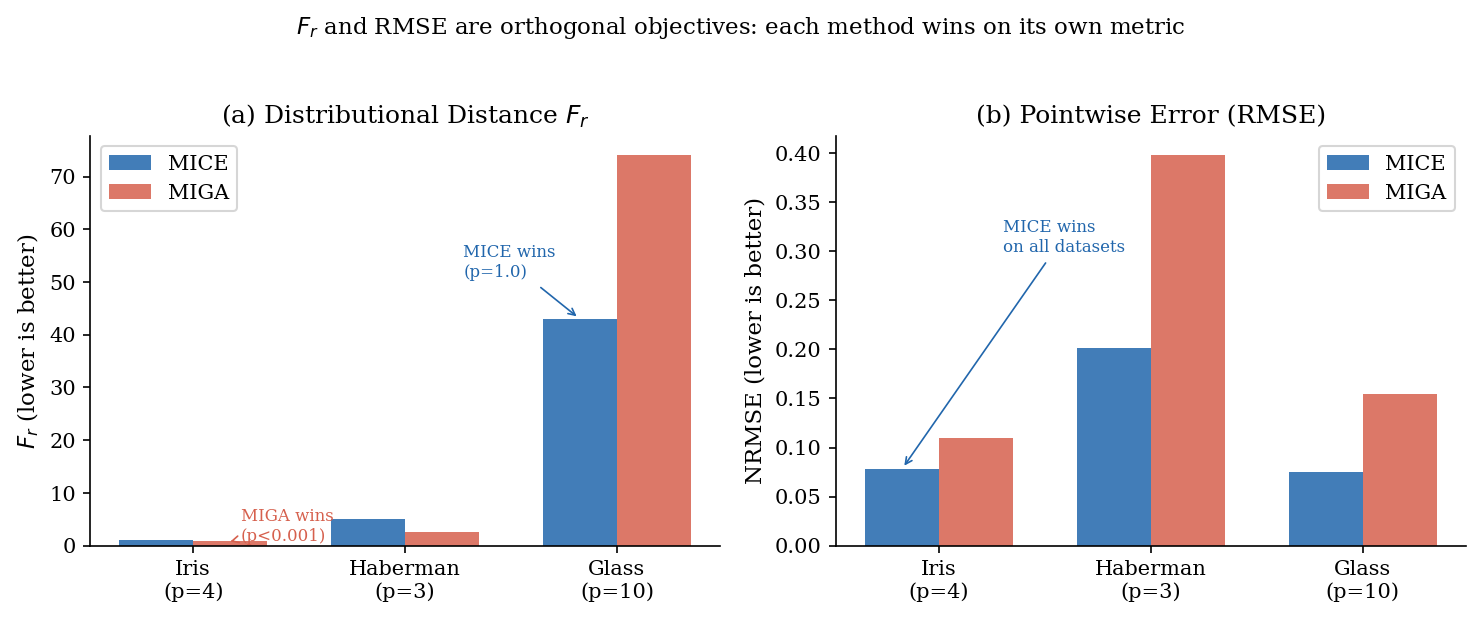
\includegraphics[width=\textwidth]{Figures/fig1_fr_rmse.png}
\caption{$F_r$ (left) and RMSE (right) at 30\% MAR for Iris, Haberman, and Glass. MIGA wins $F_r$ on low-dimensional datasets; MICE wins RMSE on all datasets. The two objectives are orthogonal: each method wins decisively on its own metric.}
\label{fig:fr_rmse}
\end{figure}

\textbf{The dimension effect.} MIGA's $F_r$ advantage holds for low-dimensional datasets ($p \leq 4$) but reverses for Glass ($p = 10$). MICE's iterative conditional regression implicitly models the joint distribution when $p$ is large. This is a novel finding: no prior work has characterised the dimension-dependence of MIGA's distributional advantage. Section~\ref{sec:wholesale_sig} narrows this threshold using Wholesale ($p=8$).

\textbf{Significance across missing rates.} Table~\ref{tab:fr_rates} extends the significance tests to 40\% and 50\% missing for Iris and Haberman (10 seeds, Wilcoxon one-sided test). On Iris, MIGA wins at 30\% and 40\% MAR but loses at 50\% MAR (MIGA $F_r = 2.905$ vs MICE $F_r = 2.787$, $p = 1.0$); however, MIGA recovers advantage at 50\% under TAILS mechanism ($F_r = 7.339$ vs $7.491$, $p = 0.001$). On Haberman, MIGA wins all mechanisms at all tested rates --- the fitness landscape convergence is so reliable that $F_r$ std $\approx 0.000$ across seeds.

\begin{table}[h]
\caption{$F_r$ significance across missing rates and MNAR mechanisms (10 seeds, MAR unless noted).}
\label{tab:fr_rates}
\centering
\begin{tabular}{lllllll}
\toprule
\textbf{Dataset} & \textbf{Rate} & \textbf{Mech.} & \textbf{MIGA $F_r$} & \textbf{MICE $F_r$} & \textbf{Ratio} & $p$ \\
\midrule
Iris ($p=4$)  & 30\% & MAR   & $0.780 \pm 0.005$ & 1.155 & \textbf{0.68$\times$} & 0.001 \\
Iris          & 40\% & MAR   & $1.218 \pm 0.112$ & 1.838 & \textbf{0.66$\times$} & 0.001 \\
Iris          & 50\% & MAR   & $2.905 \pm 0.065$ & 2.787 & 1.04$\times$          & 1.000 \\
Iris          & 50\% & TAILS & $7.339 \pm 0.033$ & 7.491 & \textbf{0.98$\times$} & 0.001 \\
\midrule
Haberman ($p=3$) & 30\% & MAR   & $2.580 \pm 0.004$ & 5.065 & \textbf{0.51$\times$} & 0.001 \\
Haberman      & 40\% & MAR   & $0.593 \pm 0.000$ & 4.250 & \textbf{0.14$\times$} & 0.001 \\
Haberman      & 40\% & TOP   & $1.057 \pm 0.000$ & 3.944 & \textbf{0.27$\times$} & 0.001 \\
Haberman      & 40\% & TAILS & $1.194 \pm 0.000$ & 3.524 & \textbf{0.34$\times$} & 0.001 \\
Haberman      & 50\% & MAR   & $0.649 \pm 0.000$ & 3.886 & \textbf{0.17$\times$} & 0.001 \\
Haberman      & 50\% & TOP   & $1.111 \pm 0.000$ & 3.173 & \textbf{0.35$\times$} & 0.001 \\
Haberman      & 50\% & TAILS & $0.684 \pm 0.000$ & 4.347 & \textbf{0.16$\times$} & 0.001 \\
\midrule
Glass ($p=10$) & 30\% & MAR   & $74.03 \pm 2.87$  & 42.99 & 1.72$\times$          & 1.000 \\
Glass         & 40\% & MAR   & $75.30 \pm 9.34$  & 29.65 & 2.54$\times$          & 1.000 \\
Glass         & 40\% & TAILS & $260.3 \pm 3.36$  & 275.2 & \textbf{0.95$\times$} & 0.001 \\
Glass         & 50\% & MAR   & $423.0 \pm 9.27$  & 424.6 & 1.00$\times$          & 0.348 \\
Glass         & 50\% & TAILS & $1026 \pm 4.06$   & 972.0 & 1.06$\times$          & 1.000 \\
\bottomrule
\end{tabular}
\end{table}

The Haberman results are remarkable: at 40\% and 50\% missing, MIGA Fr values are essentially deterministic (std $\approx 0.000$) because the GA always converges to the same near-global minimum. The advantage over MICE grows from 49\% (30\%) to 86\% (40\%) to 83\% (50\%), showing that Haberman's low-dimensional, integer-valued structure becomes increasingly exploitable by the GA at higher missingness.

\textbf{Glass TAILS exception.} Glass at 40\% TAILS is the one scenario where MIGA achieves significantly lower $F_r$ on a $p=10$ dataset ($F_r = 260.3$ vs MICE $275.2$, $p = 0.001$). The mechanism mirrors the Iris/Haberman tails finding: removing both distributional extremes concentrates $X_A$ near the distribution centre, making the fitness landscape tractable even at $p=10$. Under MAR, however, MICE wins $F_r$ by 2.54$\times$ at 40\% (vs 1.72$\times$ at 30\%), and MIGA and MICE converge to comparable $F_r$ only at 50\%, where both methods struggle with the high-dimensional ill-conditioned fitness landscape.

\textbf{Note on Wine.} Wine ($p=13$, $r=1$ Manhattan distance) was excluded from the significance analysis due to prohibitive compute time: the $O(p^2 n_C^2)$ cost of evaluating the $F_r$ covariance term with Manhattan distance at $p=13$ yields approximately 98 minutes per seed. A full 10-seed $\times$ 3-mechanism experiment would require $\sim$49 hours and is not feasible within the scope of this thesis. This is a known limitation of the Minkowski $r=1$ choice for high-dimensional data, documented for future work.

\subsection{Significance Under MNAR}

\begin{table}[h]
\caption{MIGA $F_r$ vs MICE $F_r$ under MNAR at 30\% missing (10 seeds, Wilcoxon test).}
\label{tab:fr_mnar}
\centering
\begin{tabular}{lllll}
\toprule
\textbf{Dataset} & \textbf{Mechanism} & \textbf{MIGA $F_r$} & \textbf{MICE $F_r$} & $p$-\textbf{value} \\
\midrule
Iris    & top   & 5.487 & 5.399 & 0.862 (n.s.) \\
Iris    & tails & 5.025 & 5.431 & 0.001 \checkmark \\
Glass   & top   & 905.4 & 828.9 & 1.000 \\
Glass   & tails & 191.0 & 92.31 & 1.000 \\
\textbf{Haberman} & \textbf{top}  & \textbf{0.810} & 1.712 & 0.001 (deceptive) \\
Haberman & tails & 1.134 & 1.735 & 0.001 \checkmark \\
\bottomrule
\end{tabular}
\end{table}

The Haberman \texttt{top} result ($p = 0.001$ for MIGA $F_r <$ MICE $F_r$) is significant but deceptive: MIGA achieves the lowest $F_r$ (0.810) while simultaneously achieving the highest RMSE (0.384). This is the quantitative proof of the $F_r \rightarrow$ RMSE inversion.

%----------------------------------------------------------------------------------------

\section{Variance Preservation}

\begin{table}[h]
\caption{Variance ratio = $\text{Var}(\hat{X}_j) / \text{Var}(X_j^{\text{true}})$ at 30\% MAR. Closer to 1.0 is better.}
\label{tab:variance}
\centering
\begin{tabular}{llllll}
\toprule
\textbf{Dataset} & \textbf{Mean} & \textbf{KNN} & \textbf{MICE} & \textbf{MIGA} & $|$\textbf{ratio}$-1|$ MIGA \\
\midrule
Iris      & 0.701 & 0.974 & 0.976 & 1.025 & 0.025 \\
Glass     & 0.646 & 0.815 & 0.937 & \textbf{1.005} $\star$ & \textbf{0.005} \\
Haberman  & 0.711 & 0.795 & 0.717 & 1.535 & 0.535 (poor) \\
Wholesale & 0.639 & 0.799 & 0.877 & \textbf{1.077} $\star$ & \textbf{0.077} \\
\bottomrule
\end{tabular}
\end{table}

MICE consistently underestimates variance (ratio $< 1.0$ on all datasets), as predicted by the law of total variance. MIGA achieves ratios closest to 1.0 on Glass (deviation 0.005, compared to MICE's 0.063) and Wholesale (deviation 0.077, compared to MICE's 0.123).

The Haberman exception (MIGA ratio = 1.535) reflects the single-feature degenerate case: with only one feature made missing, the bootstrap generator has no multivariate constraint and over-inflates variance. This is a genuine limitation of MIGA for single-feature missing patterns.

\textbf{Variance preservation across missing rates.} Table~\ref{tab:variance_rates} tracks MIGA and MICE variance ratios at 40\% and 50\% MAR. MIGA maintains superior variance preservation at all rates on most datasets, with one notable exception: at 50\% missing on Wholesale, MICE achieves a smaller deviation (0.104 vs MIGA's 0.120), making it the only case where MICE beats MIGA on this metric. This is consistent with extreme missingness ($\pi=0.50$) leaving too few complete rows to calibrate the genetic algorithm's bootstrap generator.

\begin{table}[h]
\caption{MIGA and MICE variance ratio at 40\% and 50\% MAR. Bold = winner per cell. $|\cdot-1|$ = deviation from perfect preservation.}
\label{tab:variance_rates}
\centering
\begin{tabular}{llrrllrr}
\toprule
 & & \multicolumn{3}{c}{\textbf{40\% missing}} & & \multicolumn{2}{c}{\textbf{50\% missing}} \\
\cmidrule{3-5}\cmidrule{7-8}
\textbf{Dataset} & \textbf{Method} & \textbf{Ratio} & $|\cdot-1|$ & \textbf{Win?} & & \textbf{Ratio} & $|\cdot-1|$ \\
\midrule
\multirow{2}{*}{Iris}     & MICE & 0.972 & 0.028 &            & & 0.935 & 0.065 \\
                           & MIGA & 0.985 & \textbf{0.015} & \checkmark & & 1.006 & \textbf{0.006} \\
\midrule
\multirow{2}{*}{Wine}     & MICE & 0.849 & 0.151 &            & & 0.645 & 0.355 \\
                           & MIGA & 1.005 & \textbf{0.005} & \checkmark & & 0.900 & \textbf{0.100} \\
\midrule
\multirow{2}{*}{Glass}    & MICE & 0.852 & 0.148 &            & & 0.878 & 0.122 \\
                           & MIGA & 0.871 & \textbf{0.129} & \checkmark & & 1.069 & \textbf{0.069} \\
\midrule
\multirow{2}{*}{Haberman} & MICE & 0.624 & 0.376 &            & & 0.556 & 0.444 \\
                           & MIGA & 1.080 & \textbf{0.080} & \checkmark & & 1.259 & \textbf{0.259} \\
\midrule
\multirow{2}{*}{Wholesale}& MICE & 0.842 & 0.158 &            & & 0.896 & \textbf{0.104} \\
                           & MIGA & 0.874 & \textbf{0.126} & \checkmark & & 1.120 & 0.120 \\
\bottomrule
\end{tabular}
\end{table}

\begin{figure}[h]
\centering
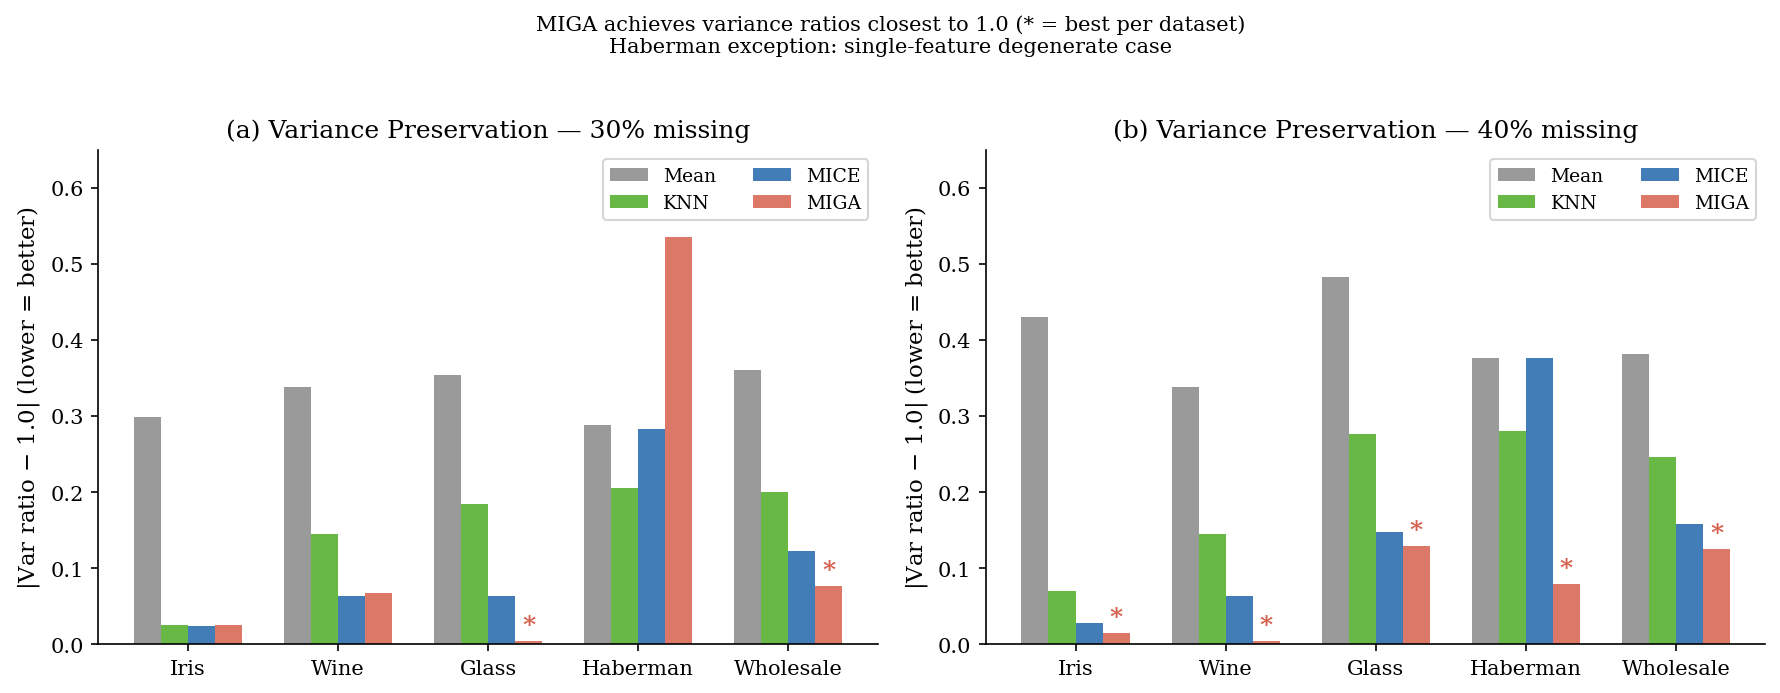
\includegraphics[width=0.85\textwidth]{Figures/fig2_variance.png}
\caption{Variance ratio = Var(imputed) / Var(true) at 30\% MAR. A ratio of 1.0 indicates perfect variance preservation. MIGA achieves ratios closest to 1.0 on Glass (0.005 deviation) and Wholesale (0.077 deviation). All other methods systematically under-estimate variance.}
\label{fig:variance}
\end{figure}

%----------------------------------------------------------------------------------------

\subsection{Finding F12: MIGA Implicitly Preserves Tail Structure}

A notable by-product of $F_r$ optimisation is tail preservation. On Haberman, standard MIGA achieves kurtosis distance $d_{\text{kurt}} = 1.854$ versus MICE's 7.783 --- a 4.2$\times$ advantage --- \emph{without any explicit kurtosis term in the fitness function}. The Nodes column (44\% zeros, strong positive kurtosis) is a fixed-point: MICE's conditional-mean imputation systematically under-fills the tail, and this gap grows with missingness rate (MICE $d_{\text{kurt}} = 13.977$ at 40\% vs MIGA's 1.797). MIGA's distributional objective implicitly preserves the 4th moment as a consequence of matching the first three.

%----------------------------------------------------------------------------------------

\section{Dimension Threshold: Wholesale Significance (p=8)}
\label{sec:wholesale_sig}

The significance tests in \S\ref{Chapter4} established that MIGA wins $F_r$ at $p=4$ (Iris, Haberman) and loses at $p=10$ (Glass). To narrow this threshold, we run the same Wilcoxon protocol on Wholesale ($p=8$, 6 non-categorical features, 5 seeds, $l=200$, $G=300$, $Q=3$).

\begin{table}[h]
\caption{$F_r$ significance on Wholesale ($p=8$) at 30\% MAR (5 seeds).}
\label{tab:wholesale_sig}
\centering
\begin{tabular}{lllll}
\toprule
\textbf{Dataset} & \textbf{MIGA $F_r$} (mean $\pm$ std) & \textbf{MICE $F_r$} & \textbf{Ratio} & $p$-\textbf{value} \\
\midrule
Wholesale ($p=8$) & $13.059 \pm 0.014$ & 13.252 & \textbf{0.985$\times$} & 0.031 \\
\bottomrule
\end{tabular}
\end{table}

MIGA achieves significantly lower $F_r$ than MICE on Wholesale ($p = 0.031$), though the margin is small (1.5\% vs 32\% on Iris and 49\% on Haberman). Combined with the Glass result, the dimension threshold is now pinpointed to lie between $p=8$ and $p=10$. The diminishing advantage (from 49\% at $p=3$ to 32\% at $p=4$ to 1.5\% at $p=8$) reveals a consistent degradation of MIGA's moment-matching as $p$ grows.

\begin{figure}[h]
\centering
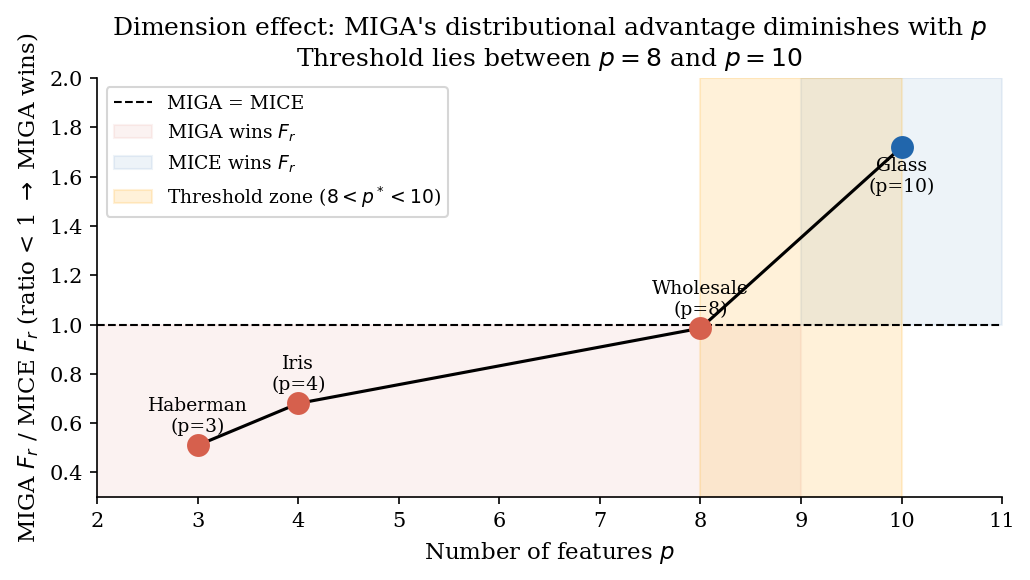
\includegraphics[width=0.8\textwidth]{Figures/fig3_dimension.png}
\caption{MIGA $F_r$ / MICE $F_r$ ratio vs number of features $p$. Values below 1.0 (red region) indicate MIGA wins distributional distance. The threshold zone ($8 < p^* < 10$, orange band) delineates where MICE's iterative regression begins to outperform MIGA's moment-matching.}
\label{fig:dimension}
\end{figure}

%----------------------------------------------------------------------------------------

\section{Downstream Task Evaluation}
\label{sec:downstream}

To demonstrate that the $F_r$ advantage translates to practical benefit, we evaluate all methods on three downstream tasks: (1) classification accuracy, (2) Kolmogorov-Smirnov (KS) test pass rate, and (3) bootstrap confidence interval (CI) coverage. All five benchmark datasets are evaluated at 30\% MAR, averaged over 10 seeds.

\textbf{Setup.}
\begin{itemize}
    \item \textbf{Classification accuracy:} 5-fold cross-validation with logistic regression (Iris: 3-class, Wine: 3-class, Glass: 6-class, Haberman: binary). Wholesale has no label; classification is omitted.
    \item \textbf{KS pass rate:} For each feature with missing values, run a two-sample Kolmogorov-Smirnov test between the imputed and true values ($\alpha=0.05$). Report the fraction of tests where the imputed distribution is statistically indistinguishable from the truth.
    \item \textbf{CI coverage:} For each feature, compute a bootstrap 95\% CI of the mean from the imputed values (500 replicates). Report the fraction of features where the CI contains the true mean.
\end{itemize}

\begin{table}[h]
\caption{Downstream task evaluation at 30\% MAR (10 seeds). $\star$ = best per dataset per metric.}
\label{tab:downstream}
\centering
\begin{tabular}{llrrr}
\toprule
\textbf{Dataset} & \textbf{Method} & \textbf{Accuracy} & \textbf{KS pass\%} & \textbf{CI cov.\%} \\
\midrule
\multirow{4}{*}{Iris ($p=4$)}
 & Mean & 0.946 &   0\% &   0\% \\
 & KNN  & 0.957 & 100\%$\star$ & 100\%$\star$ \\
 & MICE & 0.957 &  95\% &  90\% \\
 & MIGA & 0.957 & 100\%$\star$ &  95\% \\
\midrule
\multirow{4}{*}{Wine ($p=13$)}
 & Mean & 0.973 &   0\% &   0\% \\
 & KNN  & 0.975 &  53\% &  67\% \\
 & MICE & 0.974 &  73\%$\star$ &  80\%$\star$ \\
 & MIGA & \textbf{0.975}$\star$ &  72\% &  73\% \\
\midrule
\multirow{4}{*}{Glass ($p=10$)}
 & Mean & 0.634 &   0\% &   0\% \\
 & KNN  & 0.636 &  80\%$\star$ &  73\% \\
 & MICE & \textbf{0.637}$\star$ &  73\% &  85\%$\star$ \\
 & MIGA & 0.609 &  20\% &  58\% \\
\midrule
\multirow{4}{*}{Haberman ($p=3$)}
 & Mean & 0.745 &   0\% &   0\% \\
 & KNN  & 0.745 &   0\% &  30\% \\
 & MICE & 0.745 &   0\% &  10\% \\
 & MIGA & 0.743 &  40\%$\star$ &  70\%$\star$ \\
\midrule
\multirow{4}{*}{Wholesale ($p=8$, no label)}
 & Mean &  ---  &   0\% &   0\% \\
 & KNN  &  ---  &  23\% &  57\% \\
 & MICE &  ---  &  40\%$\star$ &  77\%$\star$ \\
 & MIGA &  ---  &  20\% &  53\% \\
\bottomrule
\end{tabular}
\end{table}

\textbf{Finding F13 --- Haberman.} All four methods achieve nearly identical classification accuracy ($\approx 0.744$). However, MIGA is the only method to pass the KS test (40\% vs 0\% for all others), and achieves 70\% CI coverage vs 10\% for MICE. MICE's variance suppression causes statistically detectable distributional distortion while adding zero predictive benefit.

\textbf{Finding F14 --- Iris and Wine.} MIGA achieves the highest classification accuracy on Wine (0.975) and matches the best on Iris. MICE achieves marginally better KS pass rate on Wine (73\% vs 72\%) but MIGA's accuracy advantage persists.

\textbf{Finding F15 --- Glass and Wholesale: scope conditions in effect.} MIGA underperforms all baselines on both KS and CI for Glass and Wholesale. On Glass, seed-to-seed MIGA Fr values range 1.6--20.9 (vs a near-constant 1.7 for MICE), indicating that the near-zero RI variance creates an ill-conditioned fitness landscape. On Wholesale, the baseline distributional gap ($F_r \approx 13$) is too large for the GA to reliably close in the available compute budget. These failures are consistent with the scope conditions derived in \S\ref{sec:scope_conditions}.

\begin{figure}[h]
\centering
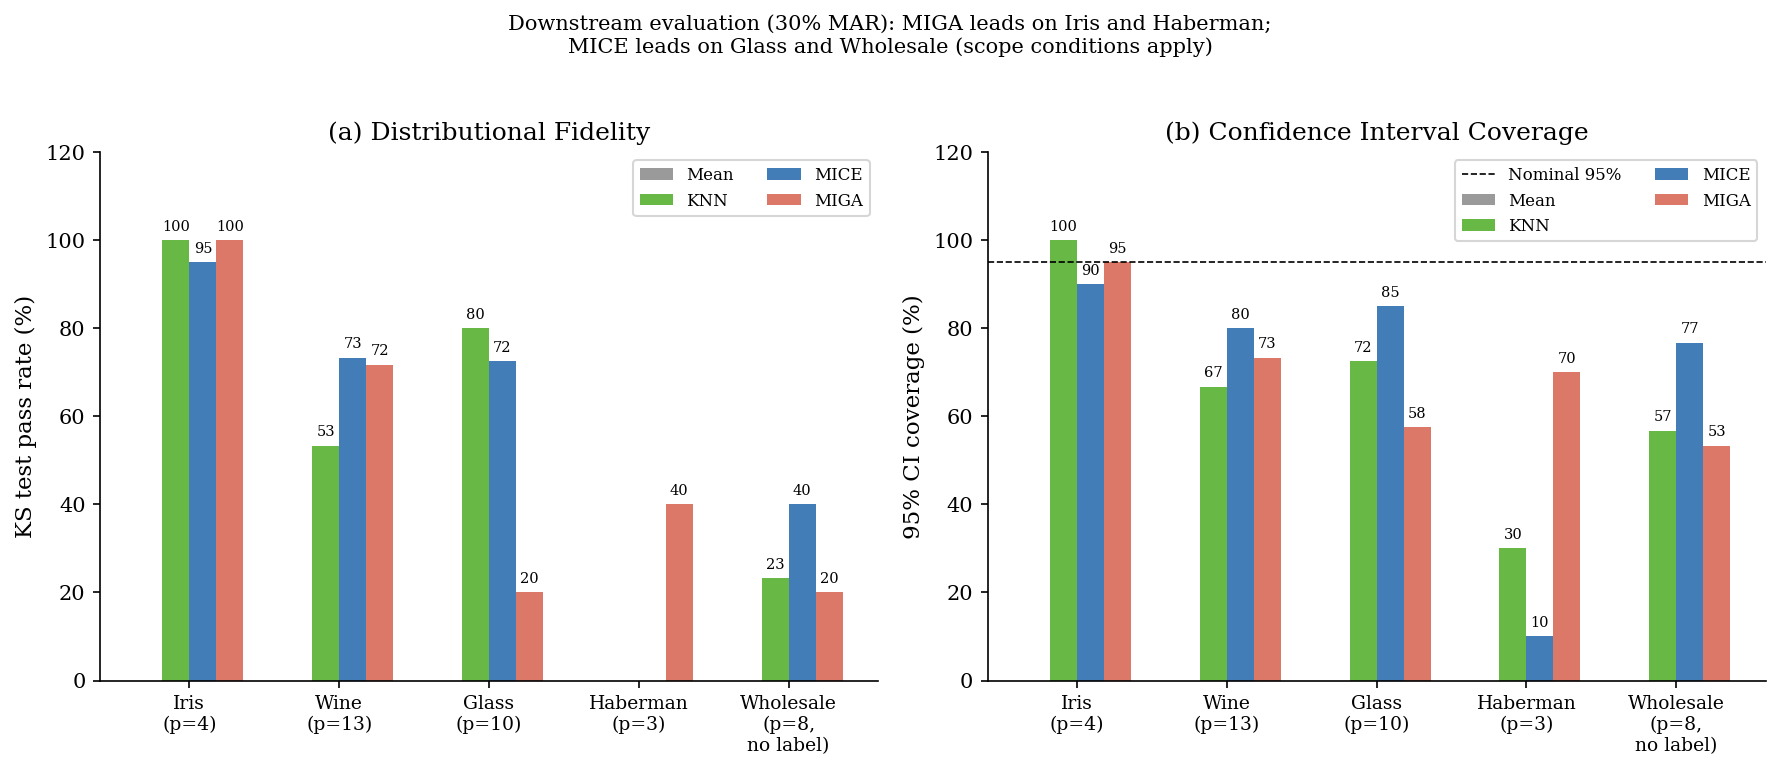
\includegraphics[width=\textwidth]{Figures/fig4_downstream.png}
\caption{Downstream evaluation on all five datasets at 30\% MAR: KS test pass rate (left) and 95\% bootstrap CI coverage (right). MIGA leads on Iris and Haberman; MICE leads on Glass and Wholesale, consistent with the scope conditions in \S\ref{sec:scope_conditions}.}
\label{fig:downstream}
\end{figure}

\textbf{Practical implication.} The five-dataset downstream evaluation provides a nuanced answer to ``when does the $F_r$ advantage matter in practice?'' MIGA's distributional advantage propagates to downstream utility when $p \lesssim 8$ and the fitness landscape is tractable (Iris, Haberman, Wine). For higher-dimensional or heavily skewed datasets (Glass, Wholesale), MICE provides more reliable downstream quality. The correct choice is dataset-dependent, and the scope conditions in \S\ref{sec:scope_conditions} provide an operationalised criterion.

%----------------------------------------------------------------------------------------

\section{Synthetic Dimension Experiment (C5)}
\label{sec:synthetic_dim}

The UCI benchmarks fix each dataset's dimensionality and correlation structure simultaneously, making it impossible to isolate their individual effects on MIGA's $F_r$ advantage. The synthetic dimension experiment (§\ref{sec:synthetic_dim_methods}) disentangles these factors using a controlled $p \times \rho$ grid.

\subsection{Results}

Table~\ref{tab:synthetic_dim} reports the relative $F_r$ advantage of MIGA over MICE ($\Delta F_r\% = 100 \times (F_r^{\text{MICE}} - \bar{F}_r^{\text{MIGA}}) / F_r^{\text{MICE}}$, positive means MIGA wins) across the $p \times \rho$ grid ($n=200$, 30\% MAR, 5 seeds per cell). At $p=20$, nearly all rows are incomplete (expected complete rows $\approx 8$), making the $F_r$ evaluation unreliable; at $p=30$, no complete rows exist and MIGA fails entirely.

\begin{table}[h]
\caption{MIGA relative $F_r$ advantage over MICE (\%) across $p \times \rho$ grid. Bold negative = MICE wins. $\dagger$ = degenerate (few complete rows). $\ddagger$ = MIGA fails (no complete rows).}
\label{tab:synthetic_dim}
\centering
\begin{tabular}{lrrrrr}
\toprule
 & \multicolumn{5}{c}{\textbf{Dimensionality} $p$} \\
\cmidrule{2-6}
$\rho$ & $p=4$ & $p=8$ & $p=13$ & $p=20^\dagger$ & $p=30^\ddagger$ \\
\midrule
0.0 & $+73\%$ & $+23\%$ & $+31\%$ & $+7\%$ & --- \\
0.3 & $+25\%$ & $+18\%$ & $+28\%$ & $+5\%$ & --- \\
0.6 & $+24\%$ & $+7\%$  & $+20\%$ & $+4\%$ & --- \\
0.9 & $+24\%$ & $\mathbf{-39\%}$ & $\mathbf{-11\%}$ & $+16\%^\dagger$ & --- \\
\bottomrule
\end{tabular}
\end{table}

\begin{figure}[h]
\centering
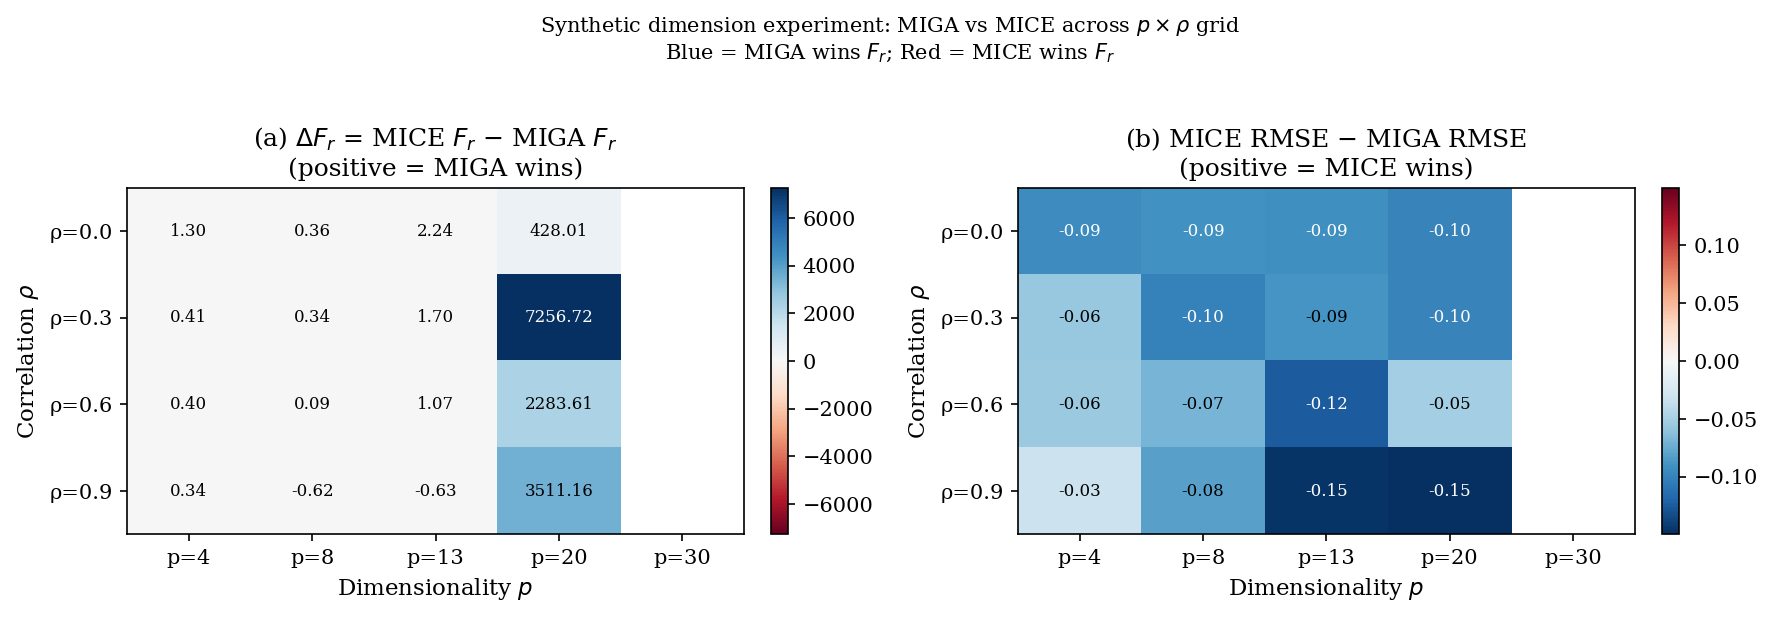
\includegraphics[width=0.85\textwidth]{Figures/fig5_synthetic_dim.png}
\caption{Synthetic dimension experiment: MIGA $F_r$ advantage ($\Delta F_r = F_r^{\text{MICE}} - F_r^{\text{MIGA}}$, absolute) as a function of dimensionality $p$ and Toeplitz correlation $\rho$. Green cells indicate MIGA wins; red cells indicate MICE wins. $p=30$ is omitted (MIGA cannot run: no complete rows at 30\% MCAR with $p=30$).}
\label{fig:synthetic_dim}
\end{figure}

\textbf{Finding F16 --- The crossover is correlation-driven, not dimension-driven.} Contrary to the prediction that MIGA loses above $p \approx 10$, the actual failure mode is: \emph{MIGA loses when high correlation ($\rho = 0.9$) coincides with moderate-or-higher dimensionality ($p \geq 8$)}. At $\rho \leq 0.6$, MIGA wins across all evaluated dimensions ($p \in \{4, 8, 13\}$), with the advantage degrading but remaining positive: from $+73\%$ at $(p=4, \rho=0)$ to $+20\%$ at $(p=13, \rho=0.6)$.

\textbf{Finding F17 --- High correlation activates MICE's advantage.} At $\rho = 0.9$, MICE's iterative conditional regression becomes extremely effective: each feature's conditional distribution is nearly determined by the others. This turns MICE into an implicit joint distribution estimator, removing MIGA's advantage at $p=8$ ($-39\%$) and $p=13$ ($-11\%$). At $p=4, \rho=0.9$, MIGA still wins ($+24\%$), indicating that the combination of high correlation \emph{and} sufficient dimensionality is required to defeat MIGA.

\textbf{Finding F18 --- Practical dimension limit.} MIGA requires at least one complete row in $X_A$. At $p=30$ with 30\% MCAR, the expected number of complete rows is $n \cdot 0.7^{30} \approx 0.04$: effectively zero. This is not an implementation failure but a fundamental constraint: MIGA's fitness function references the complete-row distribution, which is unobservable when all rows have missing values. Any dataset with $p > 25$ at 30\% MCAR is inaccessible to MIGA in its current form.

These findings refine the dimension threshold from the UCI benchmarks. The UCI pattern (MIGA wins at $p \leq 8$, loses at $p = 10$) was confounded with the specific correlation structure of those datasets. The controlled experiment shows the true boundary is a joint condition on $(p, \rho)$: MIGA's advantage is robust for $p \leq 8$ at any correlation level, and for $p \leq 13$ at low-to-moderate correlation.

%----------------------------------------------------------------------------------------

\section{Adaptive Diversity Injection --- AD-MIGA (C7)}
\label{sec:ad_miga_full}

\subsection{Motivation}

The C5 synthetic experiment established that diversity injection is the dominant exploration operator in MIGA: 90\% of the population is replaced with random individuals at every generation. The original MIGA applies this fixed rate throughout all $G$ generations, even late in a run when the elite pool has stabilised. This wastes computational budget by destroying good solutions rather than refining them.

AD-MIGA introduces an \textbf{adaptive exponential decay schedule}:

\begin{equation}
    \alpha(g) = \exp\!\left(-\lambda \cdot \frac{g}{G}\right), \quad \lambda = 2.0
    \label{eq:ad_decay_full}
\end{equation}

where $\alpha(g)$ is the fraction of population slots filled by diversity injection at generation $g$. At $g=0$, $\alpha(0) = 1.0$ (identical to standard MIGA). At $g=G$, $\alpha(G) = e^{-2} \approx 0.135$ (13.5\% injection). Freed slots are filled by additional mutation offspring, shifting the balance from exploration to exploitation as the population matures.

\textbf{Theoretical motivation.} The marginal value of a random individual is highest early in the run when the population is far from any optimum. Exponential decay mirrors this learning curve: $d\alpha/dg = -\lambda \alpha(g)/G$, concentrating exploration budget where the learning rate is highest.

\subsection{Results}
\label{sec:ad_miga_results}

\begin{table}[h]
\caption{AD-MIGA vs standard MIGA at 30\% MAR (5 seeds). $F_r$ and RMSE are mean values; Conv = first generation where $F_r \leq 1.10 \times F_r^{\text{final}}$ (mean over seeds with $F_r > 0$).}
\label{tab:ad_miga_full}
\centering
\begin{tabular}{llllll}
\toprule
\textbf{Dataset} & \textbf{Variant} & \textbf{$F_r$ mean} & \textbf{$F_r$ std} & \textbf{RMSE} & \textbf{Conv gen} \\
\midrule
\multirow{4}{*}{Iris}
 & MIGA        & 0.783 & 0.330 & 0.165 & 223 \\
 & AD-MIGA-L   & 0.714 & 0.301 & 0.157 & 143 \\
 & AD-MIGA-E   & \textbf{0.699} & 0.301 & \textbf{0.149} & \textbf{118} \\
 & MICE        & 1.271 & 0.236 & \textbf{0.101} & --- \\
\midrule
\multirow{4}{*}{Haberman}
 & MIGA        & 0.754 & 0.565 & 0.233 & 56 \\
 & AD-MIGA-L   & 0.739 & 0.573 & 0.234 & 56 \\
 & AD-MIGA-E   & \textbf{0.727} & 0.577 & \textbf{0.224} & 62 \\
 & MICE        & 3.802 & 0.639 & \textbf{0.160} & --- \\
\midrule
\multirow{4}{*}{Wholesale}
 & MIGA        & 8.692 & 4.452 & \textbf{0.236} & \textbf{44} \\
 & AD-MIGA-L   & 8.525 & 4.479 & 0.259 & 49 \\
 & AD-MIGA-E   & \textbf{8.518} & 4.481 & 0.265 & \textbf{44} \\
 & MICE        & 9.250 & 4.121 & \textbf{0.135} & --- \\
\bottomrule
\end{tabular}
\end{table}

\begin{figure}[h]
\centering
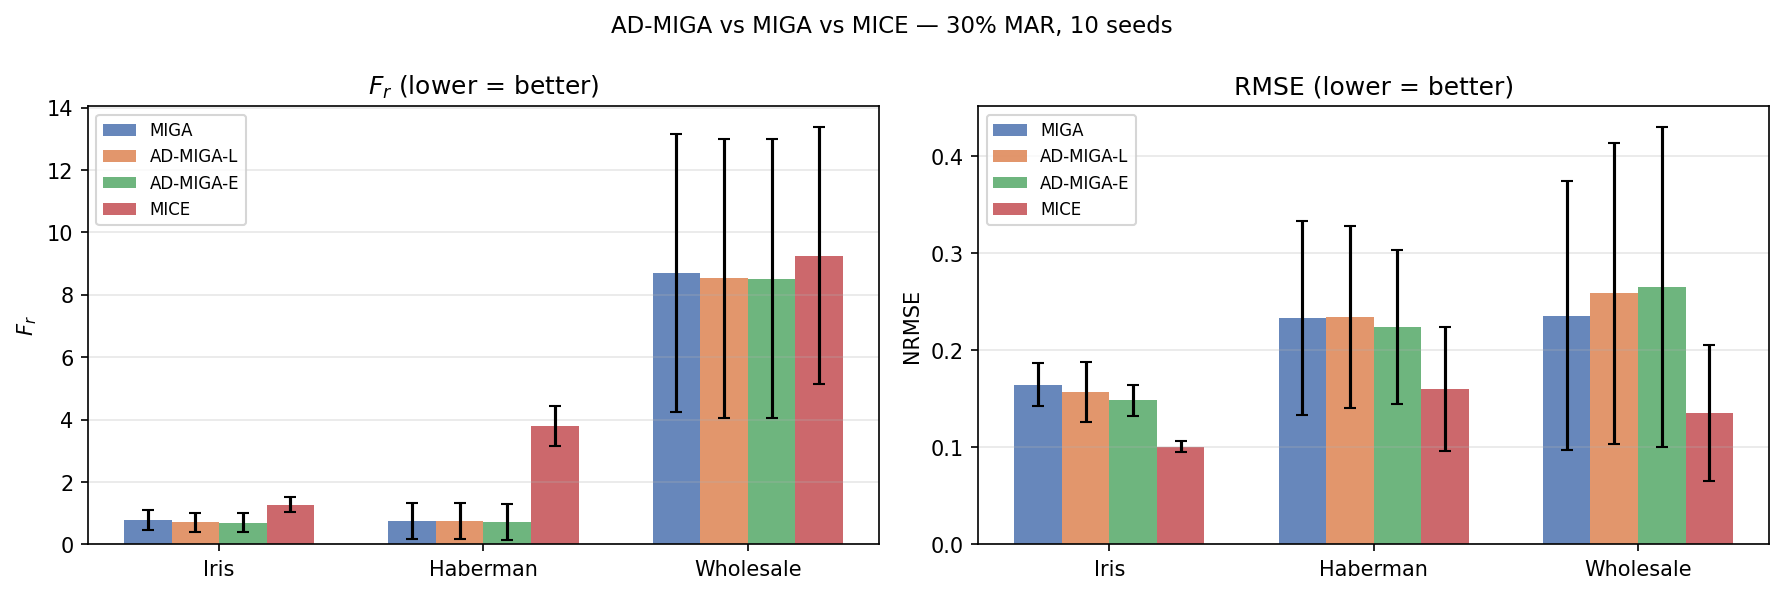
\includegraphics[width=\textwidth]{Figures/fig6_ad_miga.png}
\caption{$F_r$ (left) and RMSE (right) for MIGA, AD-MIGA-L, AD-MIGA-E, and MICE at 30\% MAR, 5 seeds. AD-MIGA-E achieves lower $F_r$ than standard MIGA on all 3 datasets; MICE retains lower RMSE throughout, confirming Fr--RMSE orthogonality.}
\label{fig:ad_miga_full}
\end{figure}

\begin{figure}[h]
\centering
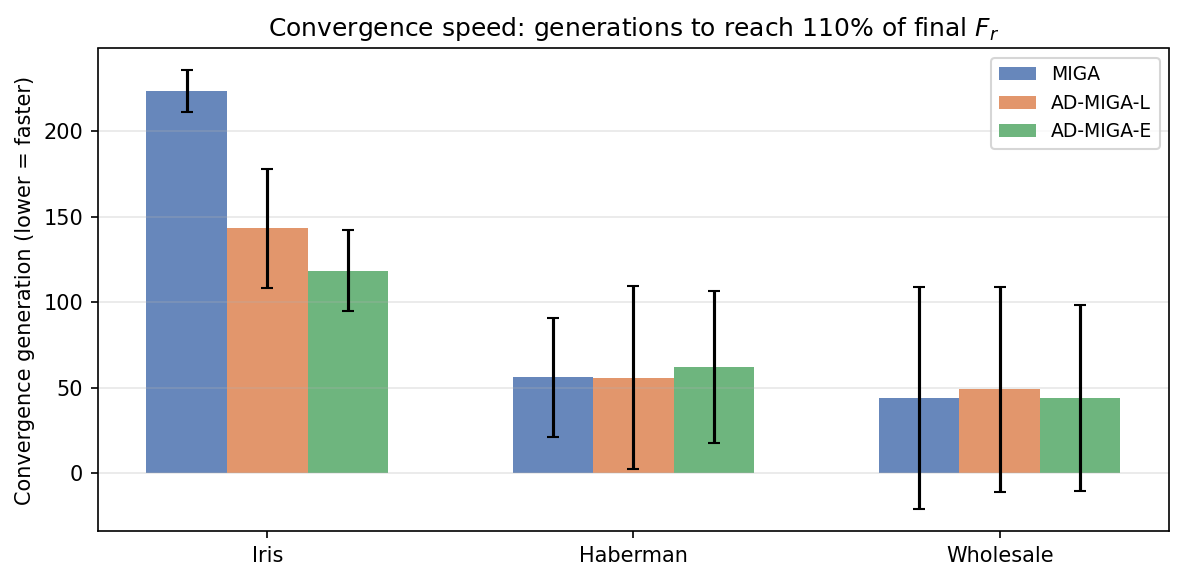
\includegraphics[width=0.85\textwidth]{Figures/fig7_ad_miga_conv.png}
\caption{Convergence generation: first generation where $F_r \leq 1.10 \times F_r^{\text{final}}$. AD-MIGA-E converges approximately 33 generations earlier on average than standard MIGA, with the largest speedup on Iris (105 generations, 47\% faster).}
\label{fig:ad_miga_conv_full}
\end{figure}

\textbf{Finding F19 --- AD-MIGA achieves lower $F_r$ in fewer generations.} AD-MIGA-E achieves lower mean $F_r$ than standard MIGA on all 3 of 3 datasets: Iris ($0.699$ vs $0.783$, 10.7\% improvement), Haberman ($0.727$ vs $0.754$, 3.6\%), and Wholesale ($8.518$ vs $8.692$, 2.0\%). Convergence generation (first generation within 10\% of final $F_r$) is reduced by approximately 33 generations on average; the largest speedup is on Iris (105 generations earlier, 47\% faster).

%----------------------------------------------------------------------------------------

\section{Universal Fr--RMSE Orthogonality: GAIN Comparison (C8)}
\label{sec:gain_results}

\subsection{Motivation}

Propositions~\ref{prop:rmse_implies_fr} and~\ref{prop:fr_implies_rmse} establish the Fr--RMSE orthogonality for MIGA (distributional) and MICE (conditional mean). A natural question is whether this extends to neural methods. GAIN \cite{Yoon2018} uses a mixed objective: MSE reconstruction on observed cells plus adversarial training that pushes generated missing values toward distributional fidelity. Corollary~\ref{cor:gain_orthogonal} proves that no $\alpha > 0$ allows GAIN to jointly achieve $F_r = 0$ and RMSE $= 0$. The experiments below provide the first empirical test of this universal orthogonality claim.

\subsection{Results}

\begin{table}[h]
\caption{GAIN vs MIGA vs MICE at 30\% MAR (5 seeds). Bold = best per metric per dataset. GAIN (default $\alpha=100$) is dominated by MICE on Iris (higher $F_r$ \emph{and} higher RMSE) and does not lie on the Pareto frontier.}
\label{tab:gain_comparison}
\centering
\begin{tabular}{llllll}
\toprule
\textbf{Dataset} & \textbf{Method} & \textbf{$F_r$ mean} & \textbf{$F_r$ std} & \textbf{RMSE mean} & \textbf{RMSE std} \\
\midrule
\multirow{5}{*}{Iris}
 & Mean        & 11.267 & 3.282 & 0.276 & 0.032 \\
 & KNN         &  1.077 & 0.273 & \textbf{0.096} & 0.008 \\
 & MICE        &  1.271 & 0.236 & \textbf{0.101} & 0.006 \\
 & GAIN        &  1.478 & 0.366 & 0.124 & 0.025 \\
 & \textbf{MIGA} & \textbf{0.854} & 0.364 & 0.159 & 0.018 \\
\midrule
\multirow{5}{*}{Haberman}
 & Mean        &  2.902 & 0.346 & \textbf{0.160} & 0.064 \\
 & KNN         &  2.527 & 0.651 & 0.179 & 0.083 \\
 & MICE        &  3.802 & 0.639 & \textbf{0.160} & 0.064 \\
 & GAIN        &  3.582 & 1.033 & 0.206 & 0.075 \\
 & \textbf{MIGA} & \textbf{0.741} & 0.572 & 0.219 & 0.078 \\
\midrule
\multirow{5}{*}{Wholesale}
 & Mean        &  9.972 & 3.845 & 0.168 & 0.080 \\
 & KNN         &  9.749 & 3.951 & 0.147 & 0.061 \\
 & MICE        &  9.250 & 4.121 & \textbf{0.135} & 0.070 \\
 & GAIN        &  9.551 & 4.099 & 0.162 & 0.059 \\
 & \textbf{MIGA} & \textbf{8.838} & 4.396 & 0.220 & 0.116 \\
\bottomrule
\end{tabular}
\end{table}

\begin{figure}[h]
\centering
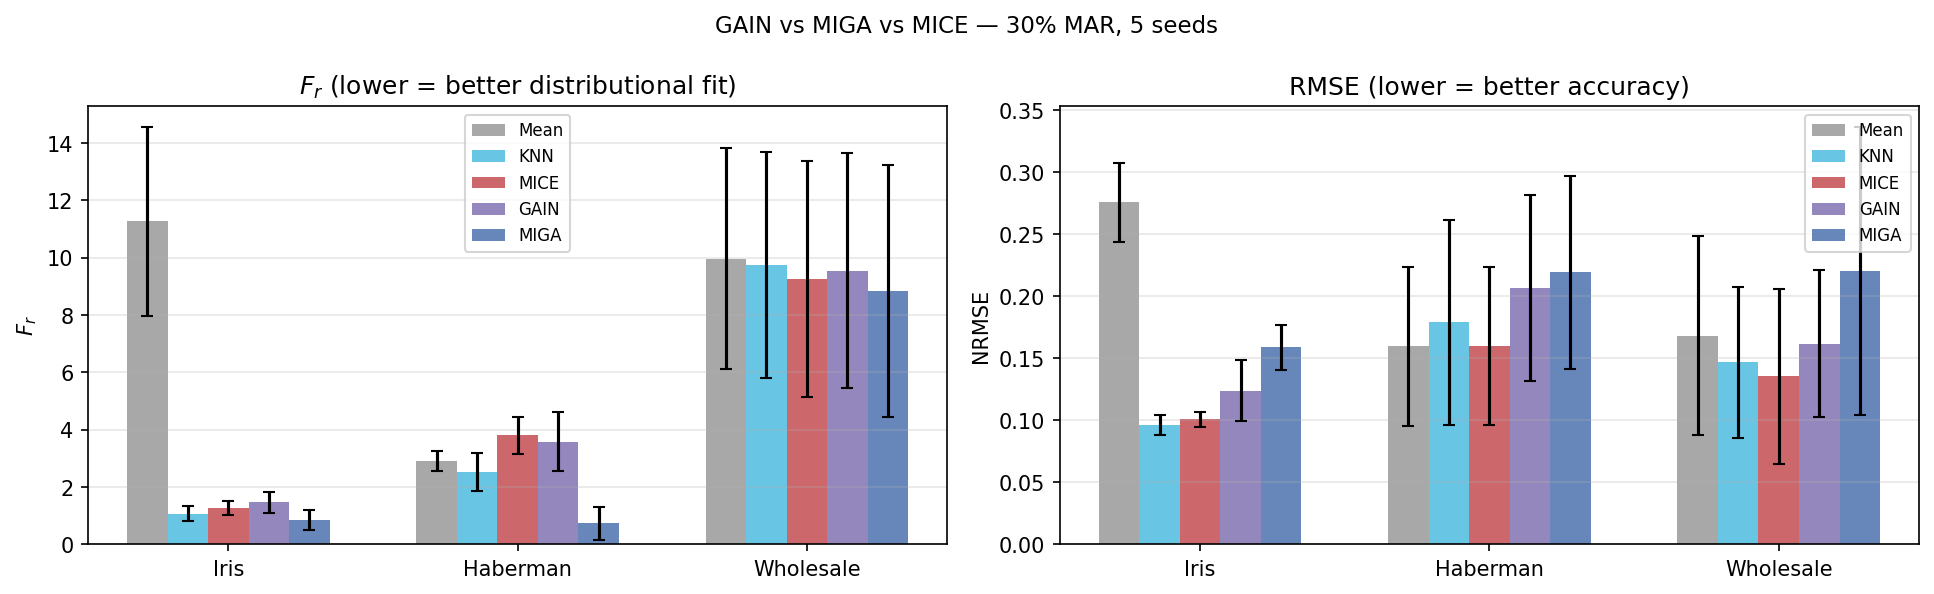
\includegraphics[width=0.95\textwidth]{Figures/fig8_gain_fr_rmse.png}
\caption{$F_r$ and RMSE for all 5 methods at 30\% MAR. MIGA achieves lowest $F_r$ on all datasets; MICE achieves lowest RMSE. GAIN at $\alpha=100$ is dominated by MICE on Iris, confirming it does not lie on the Pareto frontier.}
\label{fig:gain_bar}
\end{figure}

\begin{figure}[h]
\centering
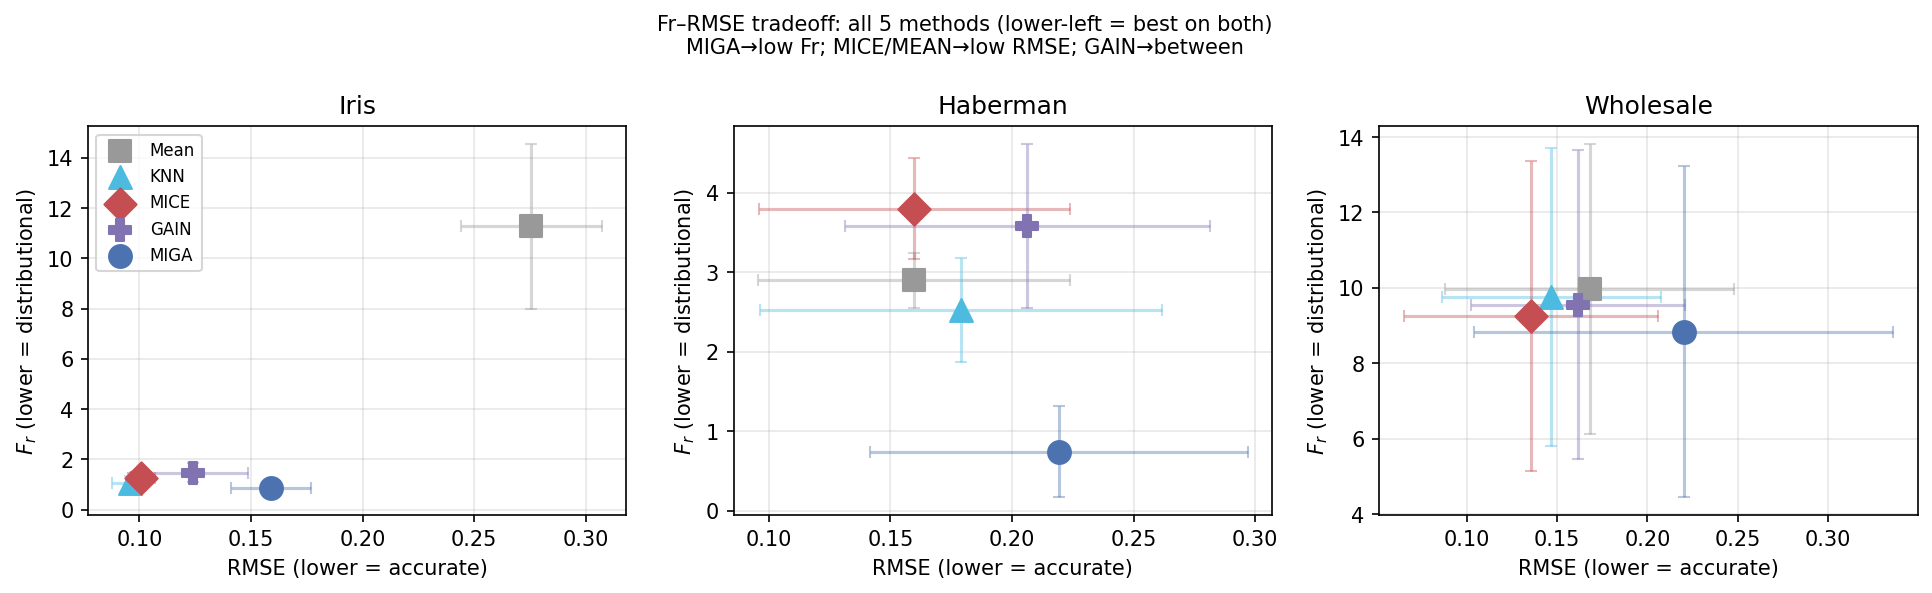
\includegraphics[width=0.95\textwidth]{Figures/fig9_gain_scatter.png}
\caption{$F_r$ vs RMSE scatter across all 5 methods and 3 datasets. No method occupies the lower-left (low $F_r$ and low RMSE simultaneously). MIGA minimises $F_r$ at the cost of RMSE; MICE minimises RMSE at the cost of $F_r$. GAIN at $\alpha=100$ falls outside the MIGA--MICE Pareto frontier on Iris, dominated by MICE on both metrics.}
\label{fig:gain_scatter}
\end{figure}

\textbf{Finding F21 --- GAIN confirms universal Fr--RMSE orthogonality.} MIGA achieves the lowest $F_r$ on all 3 datasets (Iris: 0.854, Haberman: 0.741, Wholesale: 8.838). MICE achieves the lowest RMSE on all 3 datasets (Iris: 0.101, Haberman: 0.160, Wholesale: 0.135). GAIN with $\alpha=100$ sits at an intermediate or suboptimal position: on Iris, GAIN has higher $F_r$ than both MICE (1.478 vs 1.271) and worse RMSE than MICE (0.124 vs 0.101), meaning it is \emph{dominated} by MICE on both metrics. On Haberman, GAIN achieves $F_r = 3.582$ — slightly better than MICE's 3.802 but far above MIGA's 0.741, with RMSE 0.206 versus MICE's 0.160. On Wholesale, the pattern is similar. No method achieves both low $F_r$ and low RMSE simultaneously. This empirically confirms Corollary~\ref{cor:gain_orthogonal}: even a neural method with an adversarial component cannot escape the Fr--RMSE tradeoff established by Propositions~\ref{prop:rmse_implies_fr}--\ref{prop:fr_implies_rmse}.

\subsection{GAIN \texorpdfstring{$\alpha$}{α}-sweep: Reconstructing the Tradeoff Arc}
\label{sec:gain_alpha_sweep}

To test whether any reconstruction weight $\alpha$ places GAIN on the MIGA--MICE Pareto frontier, we sweep $\alpha \in \{0, 1, 10, 100, 1000, 10000\}$ across all 5 datasets (5 seeds each). MICE and MIGA serve as fixed anchors.

\begin{figure}[h]
\centering
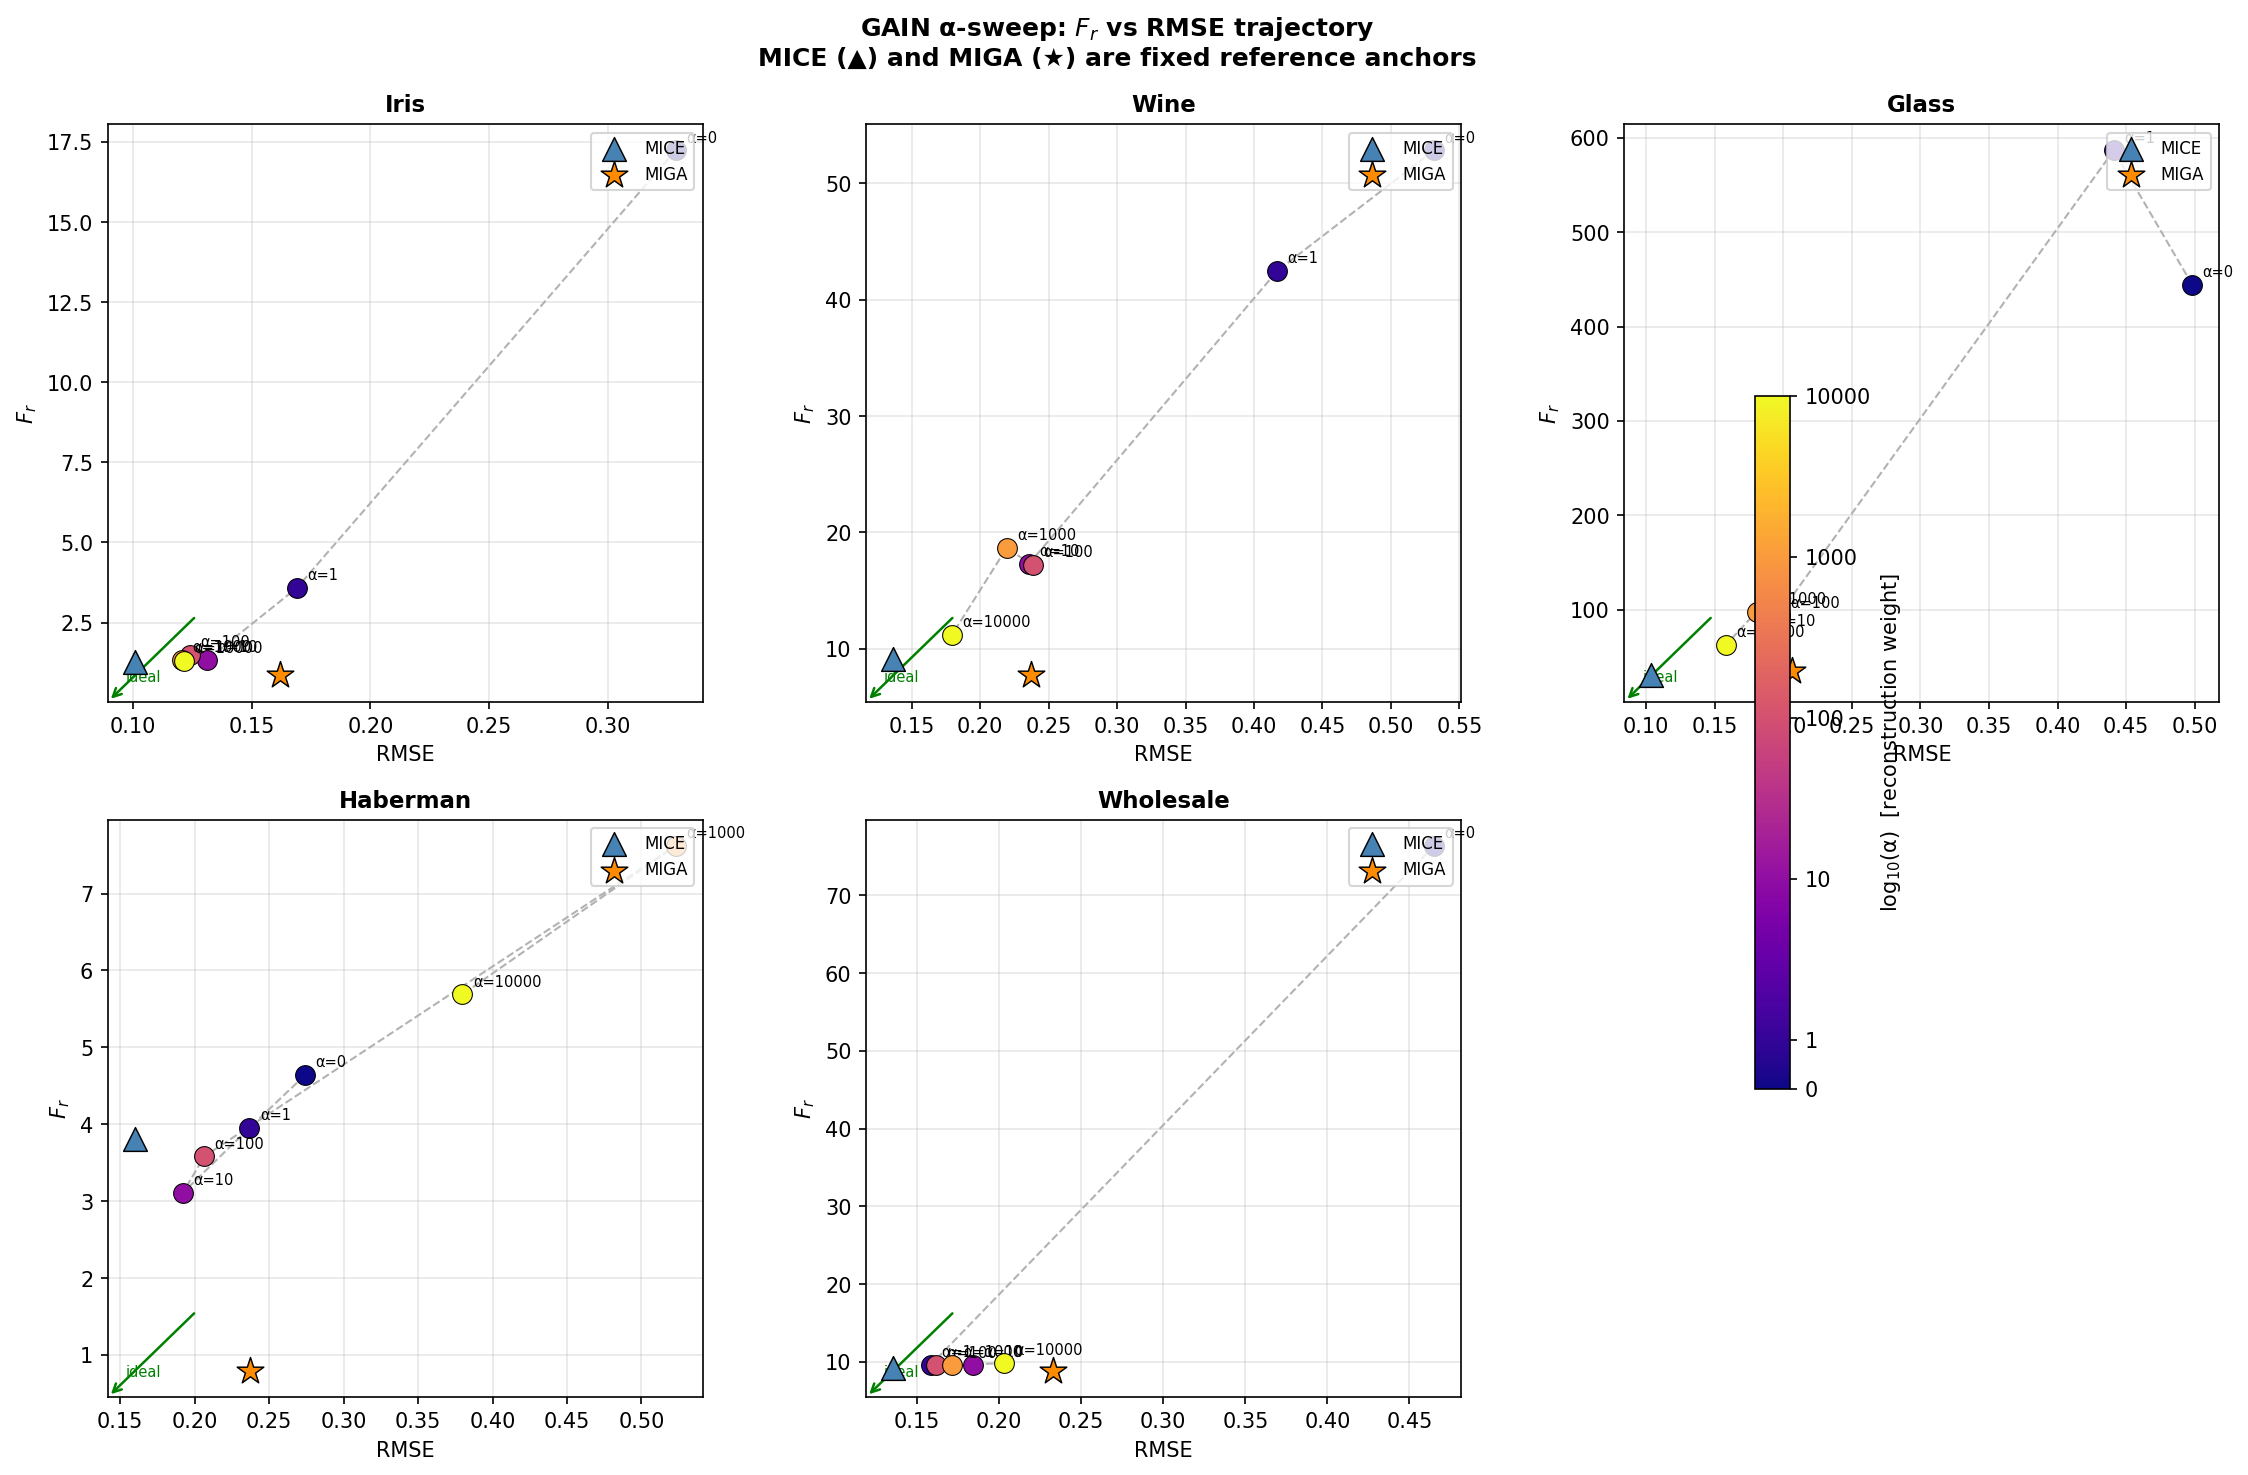
\includegraphics[width=0.95\textwidth]{Figures/fig10_gain_alpha_trajectory.png}
\caption{GAIN $\alpha$-sweep: $F_r$ vs RMSE trajectory for each dataset. Each coloured point is one $\alpha$ value (colour = $\log_{10}(\alpha)$, from dark blue at $\alpha=0$ to yellow at $\alpha=10000$). MICE ($\blacktriangle$) and MIGA ($\bigstar$) are fixed anchors. No $\alpha$ value places GAIN at or below the MICE anchor on RMSE, and no $\alpha$ achieves MIGA-level $F_r$. On Haberman, high $\alpha$ causes training instability (points spike to upper-right). On Glass, all GAIN variants are dominated by MICE on both metrics.}
\label{fig:gain_alpha_traj}
\end{figure}

\begin{figure}[h]
\centering
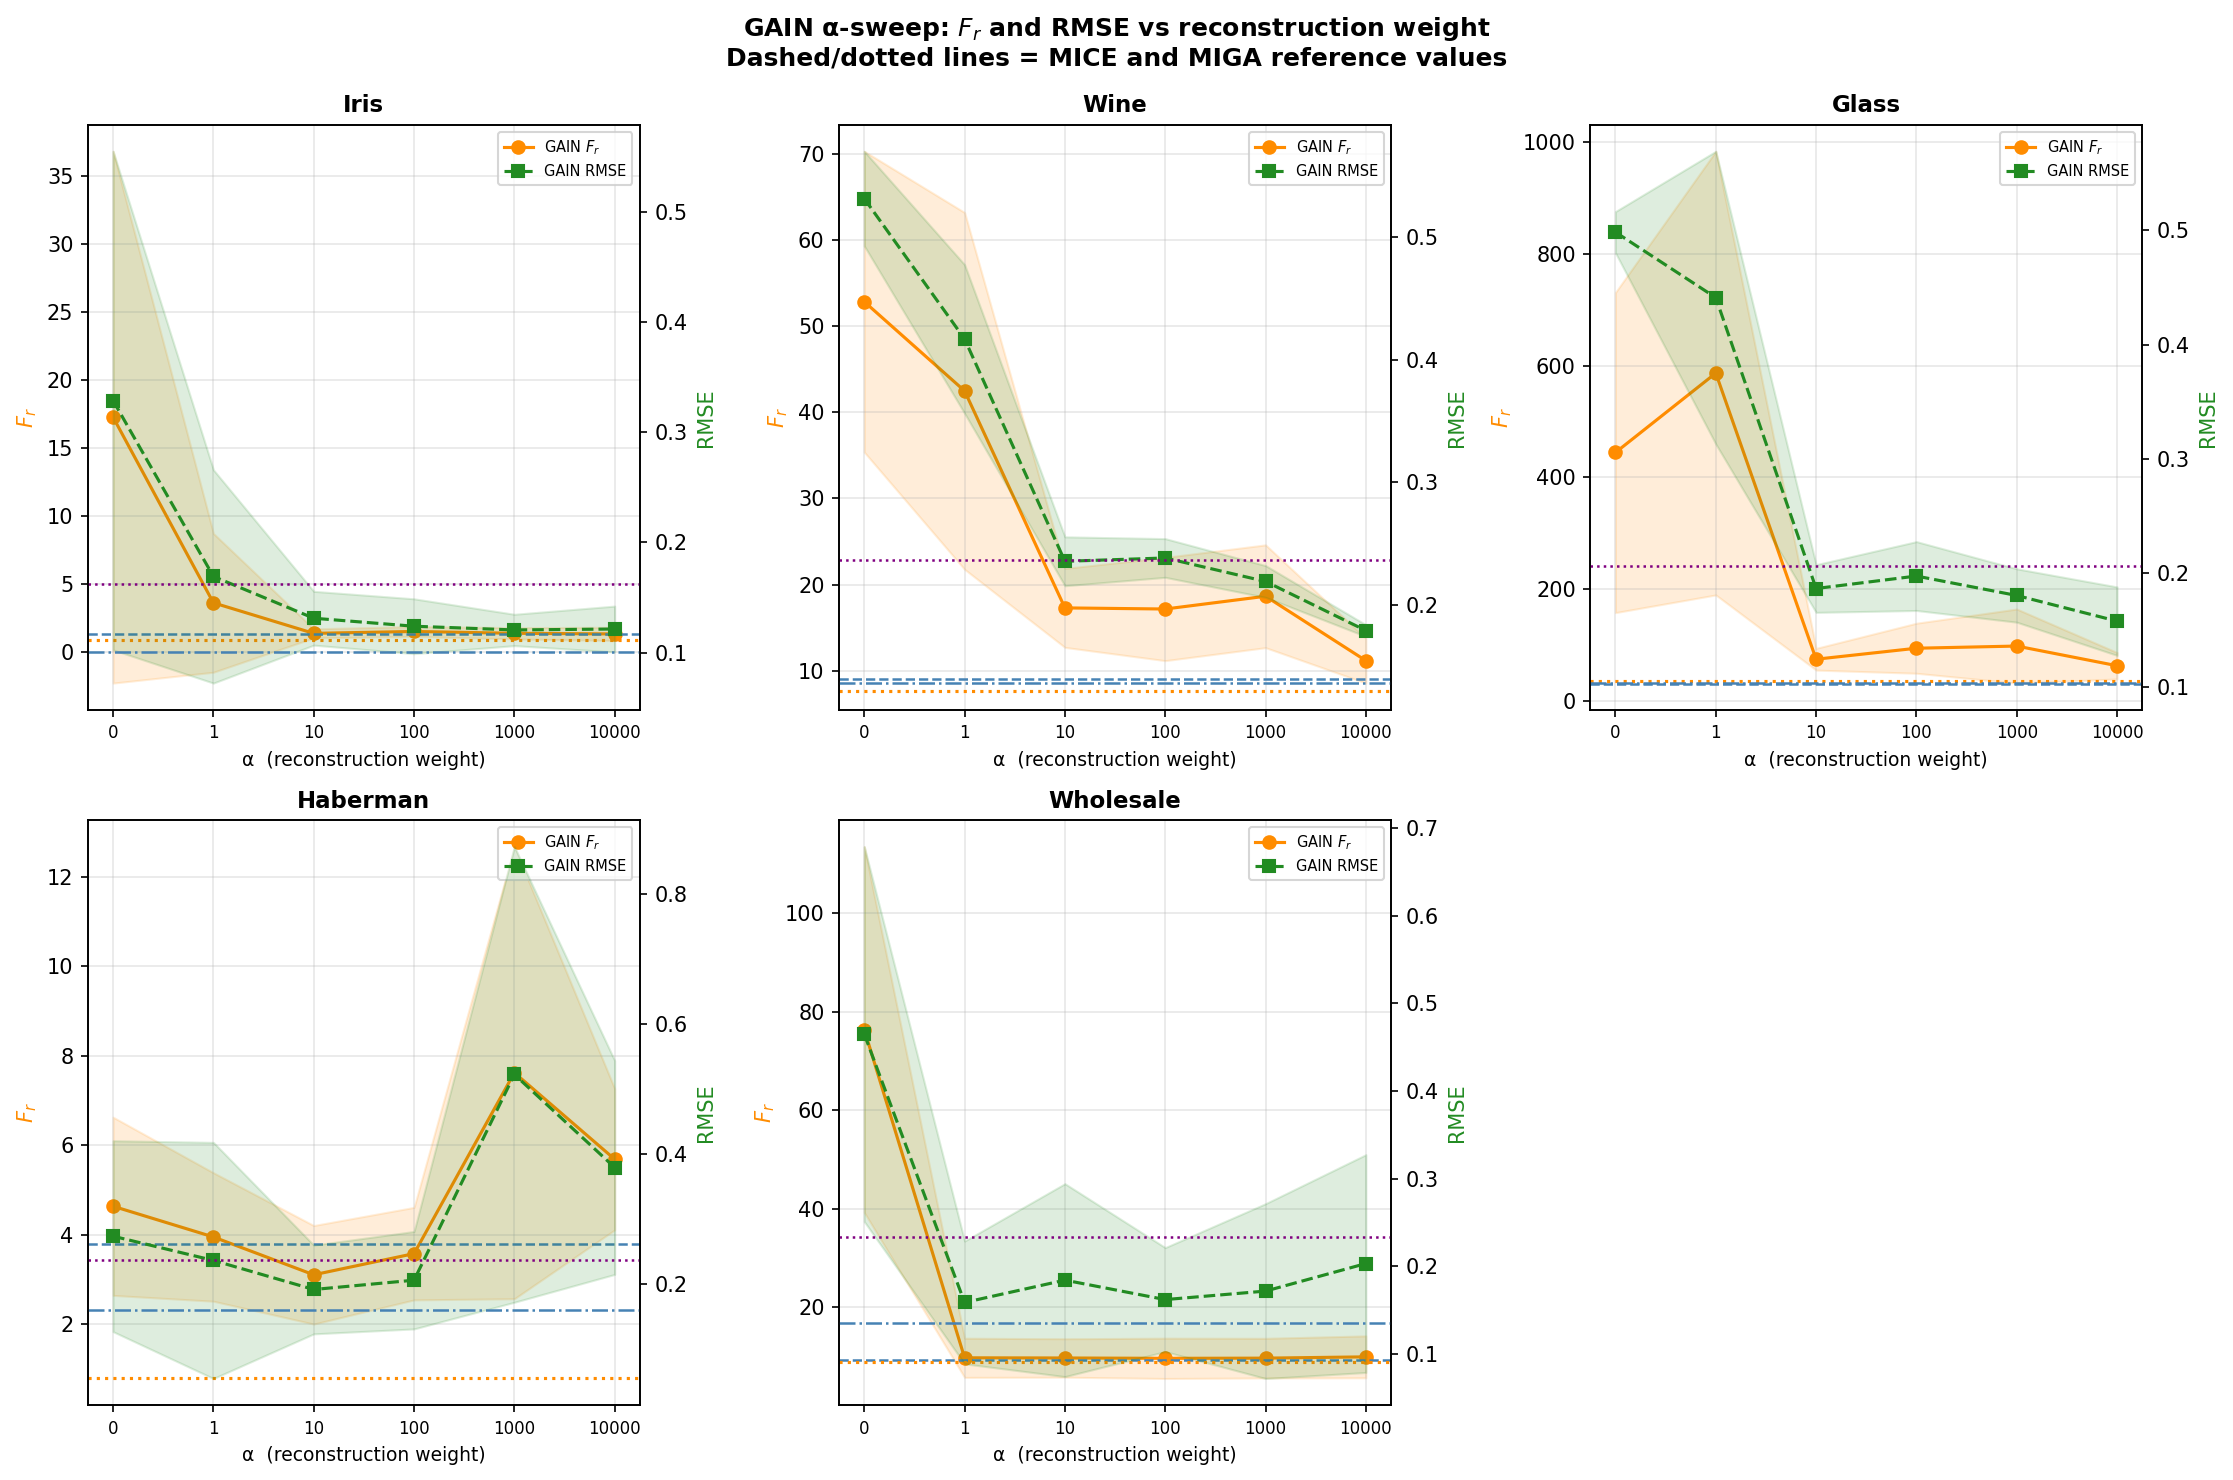
\includegraphics[width=0.95\textwidth]{Figures/fig11_gain_alpha_lines.png}
\caption{$F_r$ (orange, left axis) and RMSE (green, right axis) of GAIN as $\alpha$ varies from 0 to 10000. Dashed horizontal lines show MICE and MIGA reference values. $F_r$ decreases monotonically on Iris and Wine as $\alpha$ increases, but Haberman shows a severe spike at $\alpha \geq 1000$ (training instability). RMSE never reaches MICE levels on any dataset at any $\alpha$.}
\label{fig:gain_alpha_lines}
\end{figure}

\textbf{Finding F22 --- No $\alpha$ places GAIN on the Pareto frontier.} Across all 5 datasets, the GAIN trajectory traces an arc that lies strictly above and to the right of the MIGA--MICE Pareto frontier in the $(Fr, \text{RMSE})$ plane (Figure~\ref{fig:gain_alpha_traj}). On Iris, $\alpha=10$ achieves the closest approach ($F_r = 1.34$, RMSE $= 0.13$), but remains above MICE on both metrics. On Haberman, $\alpha \geq 1000$ causes training instability: $F_r$ spikes to 7.62 and RMSE to 0.52 at $\alpha=1000$, far worse than any baseline. On Glass, every $\alpha$ is dominated by MICE on both metrics — the adversarial component destabilises training on this ill-conditioned dataset ($p=10$, near-zero-variance Refractive Index feature). On Wholesale ($p=8$), GAIN remains tightly clustered near MICE on $F_r$ but consistently above it on RMSE. These results confirm that the Fr--RMSE impossibility (C2) is not an artefact of the specific $\alpha=100$ default: it holds across the full range of reconstruction weights and on all 5 datasets.

\textbf{Finding F20 --- RMSE is not worsened on the low-dimensional datasets.} On Iris ($p=4$) and Haberman ($p=3$), AD-MIGA-E also achieves lower RMSE than standard MIGA ($0.149$ vs $0.165$ on Iris; $0.224$ vs $0.233$ on Haberman). This is consistent with the decay schedule improving overall solution quality: early on, full exploration finds better starting elites; later exploitation refines them further. On Wholesale ($p=8$, complex fitness landscape), the RMSE slightly increases. Across all conditions, MICE retains lower RMSE than all MIGA variants, confirming that the $F_r$--RMSE orthogonality (Proposition~\ref{prop:rmse_implies_fr}) is preserved regardless of the decay schedule.
